% !TEX program = xelatex
\documentclass[11pt]{ctexbeamer}

\usetheme{Inf}

\usepackage{textcomp}
\usepackage{multicol}

\usepackage{graphicx}
\graphicspath{{figures/}}

\usepackage{fontspec}
\usepackage{moresize}

% \usepackage[no-math]{fontspec}
% \setmainfont{Times New Roman}
% \setsansfont{Arial}
% \setmonofont{Courier New}
%
% % 设定中文字体
% \usepackage[BoldFont,SlantFont,CJKchecksingle,CJKnumber]{xeCJK}
% %\setCJKmainfont[BoldFont={Adobe Heiti Std},ItalicFont={Adobe Kaiti Std}]{Adobe Song Std}
% \setCJKmainfont[BoldFont={Adobe Heiti Std},ItalicFont={Adobe Kaiti Std}]{WenQuanYi Micro Hei}
% \setCJKsansfont{Adobe Heiti Std}
% \setCJKmonofont{Adobe Fangsong Std}
% \punctstyle{hangmobanjiao}
%
% \defaultfontfeatures{Mapping=tex-text}
% \usepackage{xunicode}
% \usepackage{xltxtra}
%
% \XeTeXlinebreaklocale "zh"
% \XeTeXlinebreakskip = 0pt plus 1pt minus 0.1pt
%
% \usepackage{setspace}

%\includeonlyframes{current}



\titlegraphic{
\includegraphics[width=2.7cm]{logo_tmu.png}}
\title{\huge{生物信息学导论}}
\subtitle{\Large{$\S 4$单细胞组学与生物信息学}}
\author{\vspace{-0.6cm}\large{伊现富(Yi Xianfu)}}
% \date{\large{2022年12月23日}}
\date{\large{2022年12月30日}}
\institute{\centering{\large{基础医学院\\ 生物信息学系\vspace{0.3cm}\\ 2022-2023学年 \textbullet \ 上学期(秋)\vspace{0.1cm}\\ 生物信息学专业 \textbullet \ 2022级本科生}}}
% \logo{
\includegraphics[width=1.2cm]{logo_dbx.jpg}}


\begin{document}

\setbeamertemplate{section in toc}[circle]
\setbeamertemplate{subsection in toc}[square]
% 在每个Section前都会加入的Frame
\AtBeginSection[]
{
  \begin{frame}<beamer>
    \frametitle{教学提纲}
    \setcounter{tocdepth}{3}
    \begin{multicols}{2}
      \tableofcontents[currentsection]
    \end{multicols}
  \end{frame}
}
% 在每个Subsection前都会加入的Frame
\AtBeginSubsection[]
{
  \begin{frame}<beamer>
%%\begin{frame}<handout:0>
%% handout:0 表示只在手稿中出现
    \frametitle{教学提纲}
    \setcounter{tocdepth}{3}
    \begin{multicols}{2}
    \tableofcontents[currentsection,currentsubsection]
    \end{multicols}
  \end{frame}
}

\begin{frame}[standout]
   \begin{center}
    {\Huge 生物信息学导论\\}
    \vspace{1cm}
    {\LARGE 天津医科大学\\}
    \vspace{0.2cm}
    {\LARGE 基础医学院\\}
    \vspace{-0.1cm}
    {\LARGE 生物信息学系\\}
    \vspace{1cm}
    {\LARGE 生物信息学专业}
  \end{center}
\end{frame}

\begin{frame}
  \maketitle
\end{frame}

\begin{frame}
  %\frametitle{教学提纲}
  \begin{multicols}{2}
    \tableofcontents
  \end{multicols}
\end{frame}

\section{导言}
\subsection{常规转录组}
\begin{frame}
  \frametitle{导言 | 转录组 | 简介}
  \begin{block}{转录组}
    特定组织或细胞在某一发育阶段或功能状态下转录出来的所有RNA的集合,包括编码蛋白质的信使RNA(mRNA)和非编码RNA(rRNA、tRNA和其他ncRNAs)。\\
    转录组是连接基因组和蛋白质组遗传信息和生物功能的纽带。
  \end{block}
  \pause
  \begin{block}{转录组学}
    从整体转录水平系统研究基因转录图谱并揭示复杂生物学通路和性状调控网络分子机制的学科。
  \end{block}
  \pause
  \begin{block}{转录组测序(RNA-seq,RNA sequencing,bulk sequencing)}
利用高通量测序技术对组织或细胞中所有RNA反转录而成的cDNA文库进行测序,从整体水平研究基因的功能及其结构,揭示特定生物学过程以及疾病发生过程中的分子机制。
  \end{block}
\end{frame}
\begin{frame}
  \frametitle{导言 | 转录组 | 流程}
  \begin{figure}
    \centering
    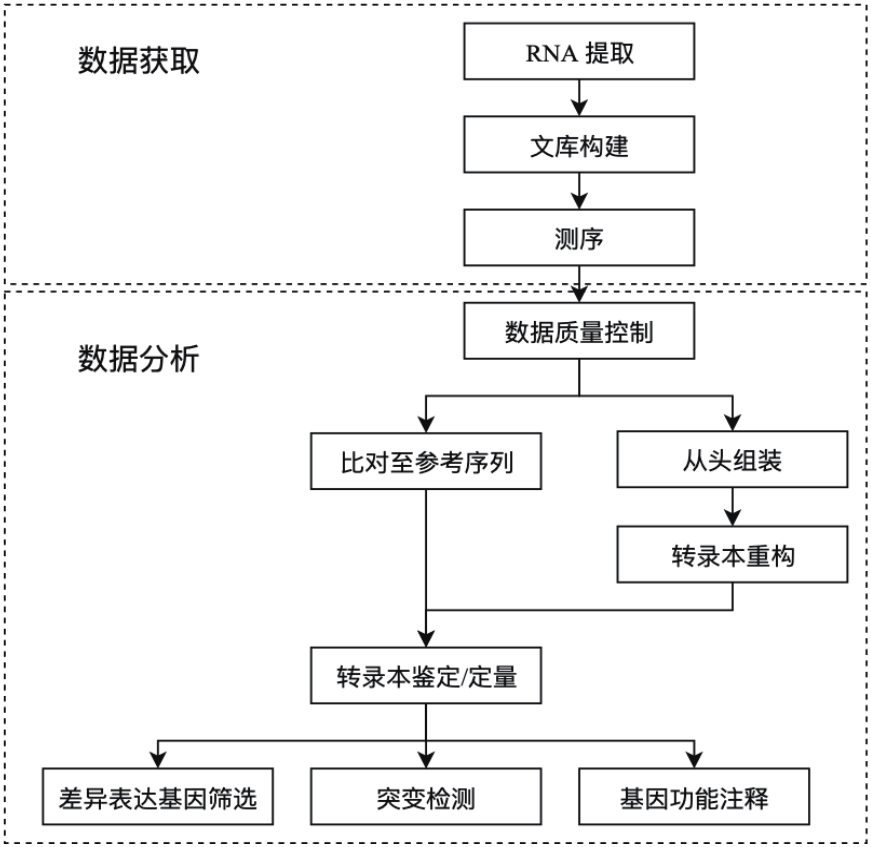
\includegraphics[width=0.4\textwidth]{RNAseq_workflow_1.png}
    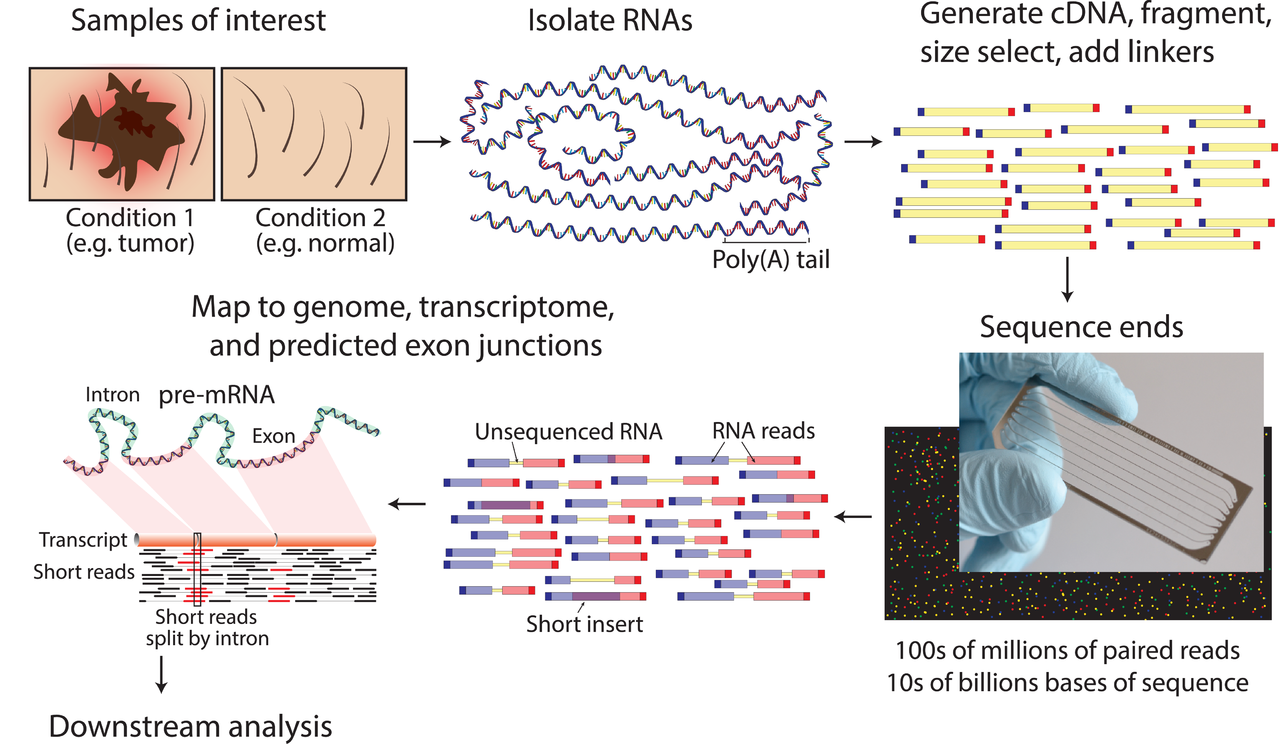
\includegraphics[width=0.55\textwidth]{RNAseq_workflow_2.png}
  \end{figure}
\end{frame}
\begin{frame}
  \frametitle{导言 | 转录组 | 流程}
  \begin{figure}
    \centering
    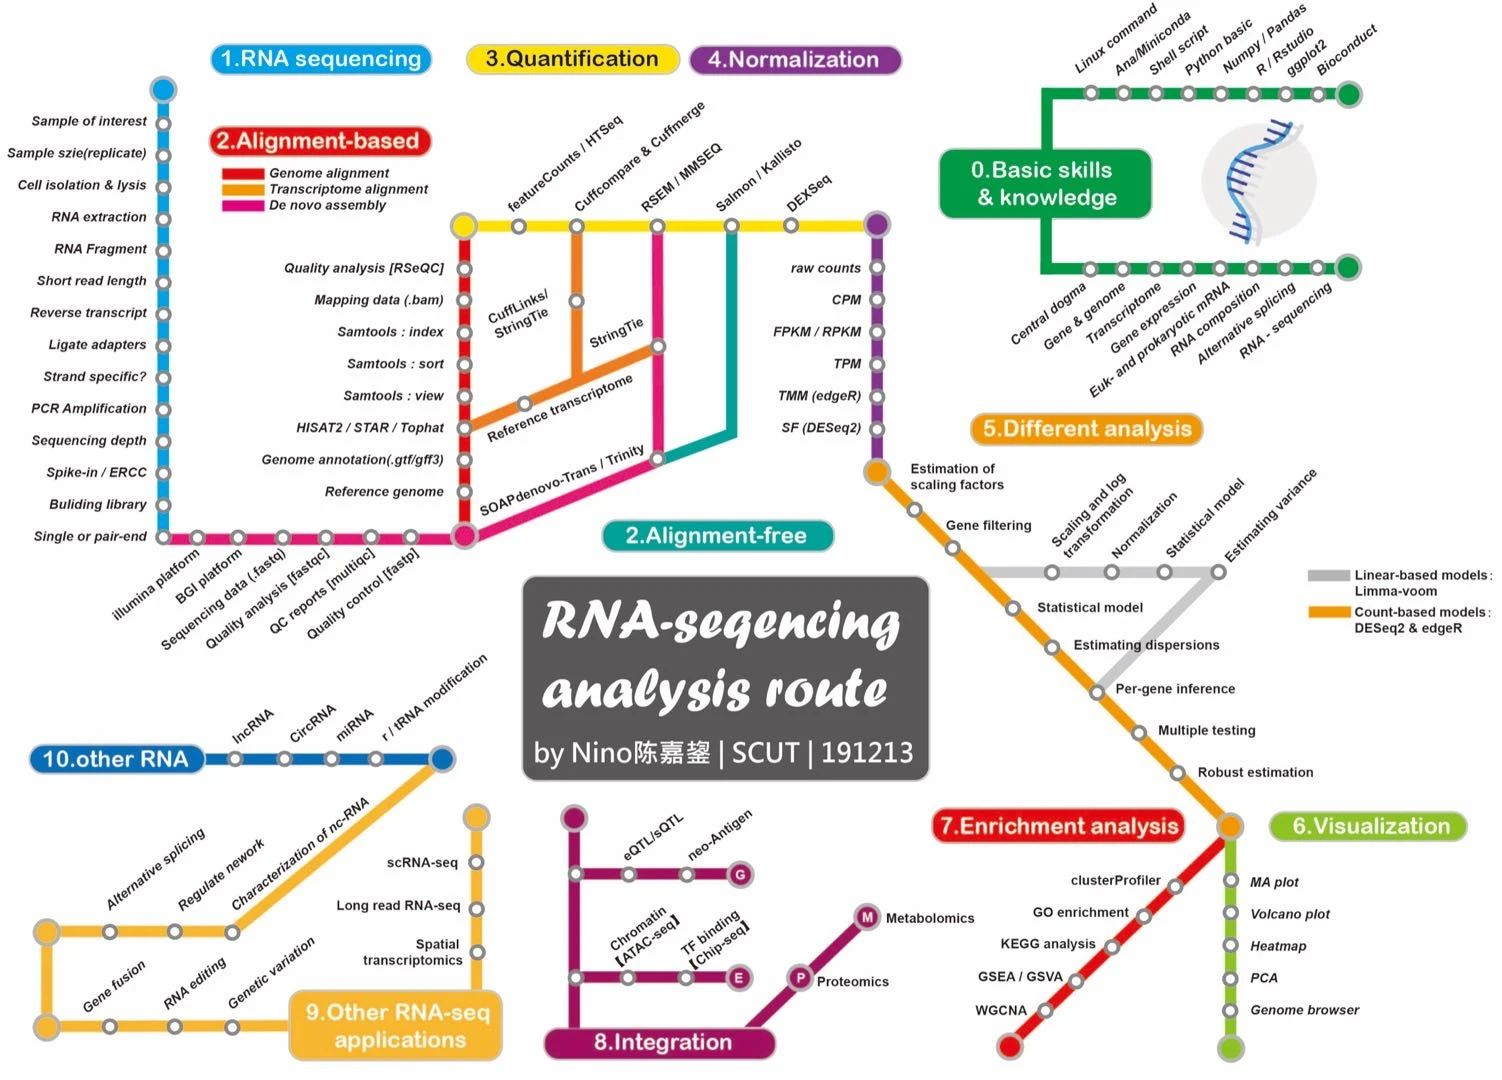
\includegraphics[width=0.95\textwidth]{RNAseq_route.png}
  \end{figure}
\end{frame}
\begin{frame}
  \frametitle{导言 | 转录组 | 应用}
  \begin{columns}
    \column{0.35\textwidth}
      \begin{block}{RNA-seq应用}
        \begin{itemize}
          \item 基因表达定量
          \item \alert{差异表达分析}
          \item 新转录本预测
          \item 可变剪接研究
          \item 共表达网络分析
          \item 变异检测
          \item 融合基因识别
          \item ……
        \end{itemize}
      \end{block}
    \column{0.65\textwidth}
  \begin{figure}
    \centering
    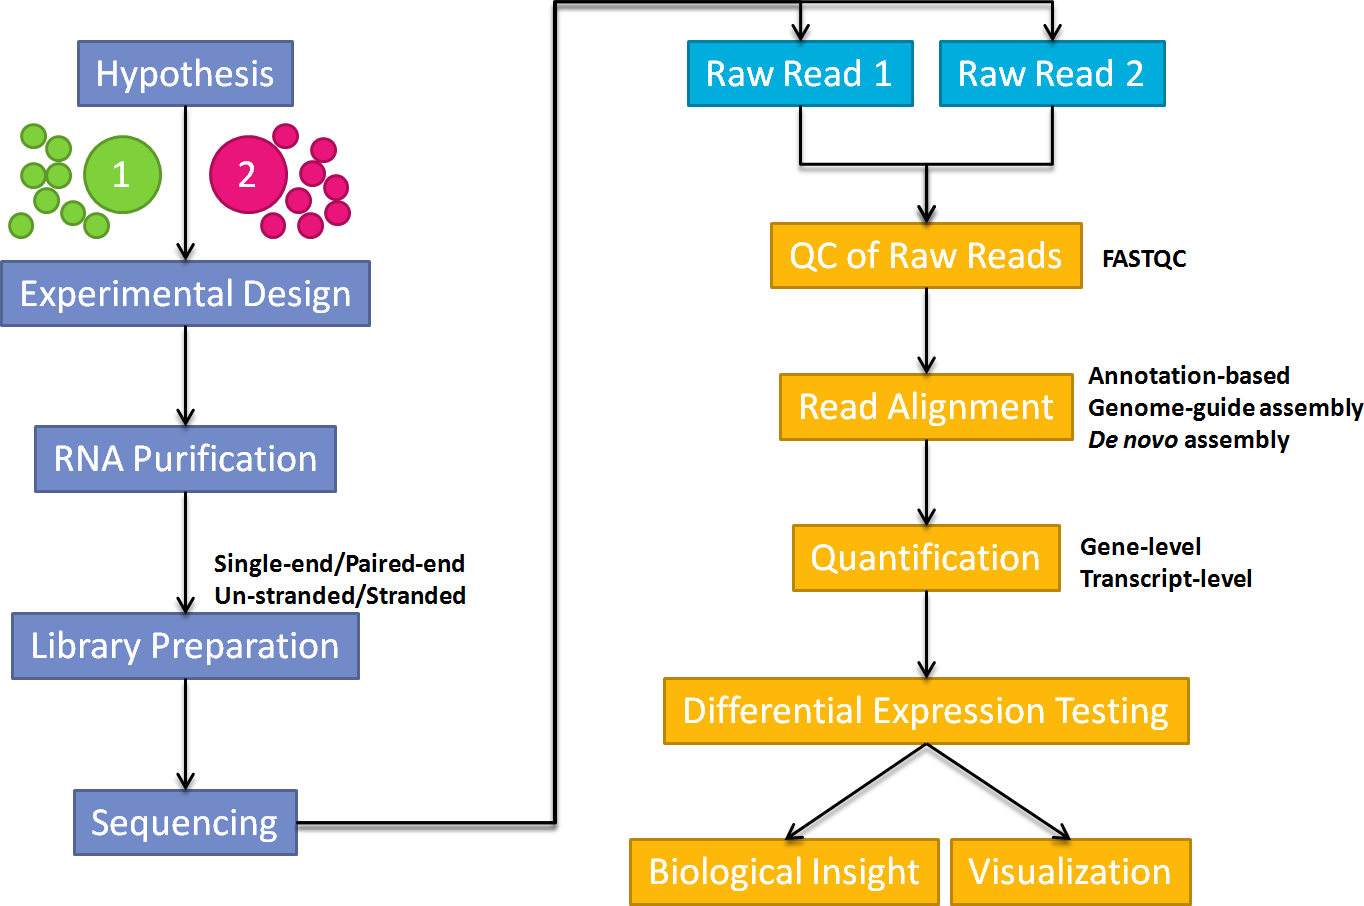
\includegraphics[width=\textwidth]{RNAseq_DEG.png}
  \end{figure}
  \end{columns}
\end{frame}
\begin{frame}
  \frametitle{导言 | 转录组 | 局限}
      \begin{block}{RNA-seq局限:异、时、空}
        \begin{itemize}
          \item \alert{组织中的细胞存在异质性} $\Longrightarrow$ 单细胞转录组(scRNA-seq)
          \item 转录是实时变化的动态过程 $\Longrightarrow$ 活细胞转录组(Live-seq)
          \item 组织中的细胞具有空间位置 $\Longrightarrow$ 空间转录组(ST)
        \end{itemize}
      \end{block}
  \begin{columns}
    \column{0.48\textwidth}
  \begin{figure}
    \centering
    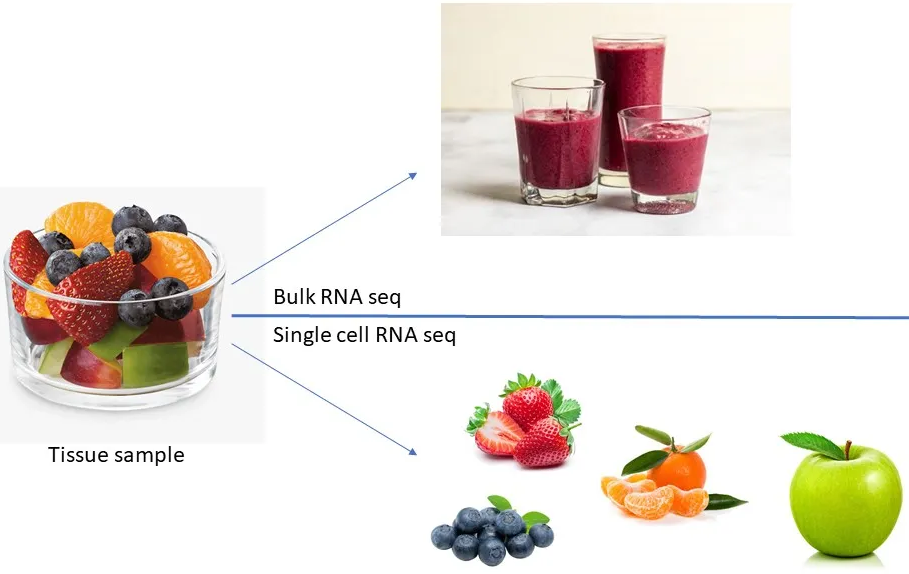
\includegraphics[width=\textwidth]{bulk_vs_sc_05.png}
  \end{figure}
    \column{0.52\textwidth}
  \begin{figure}
    \centering
    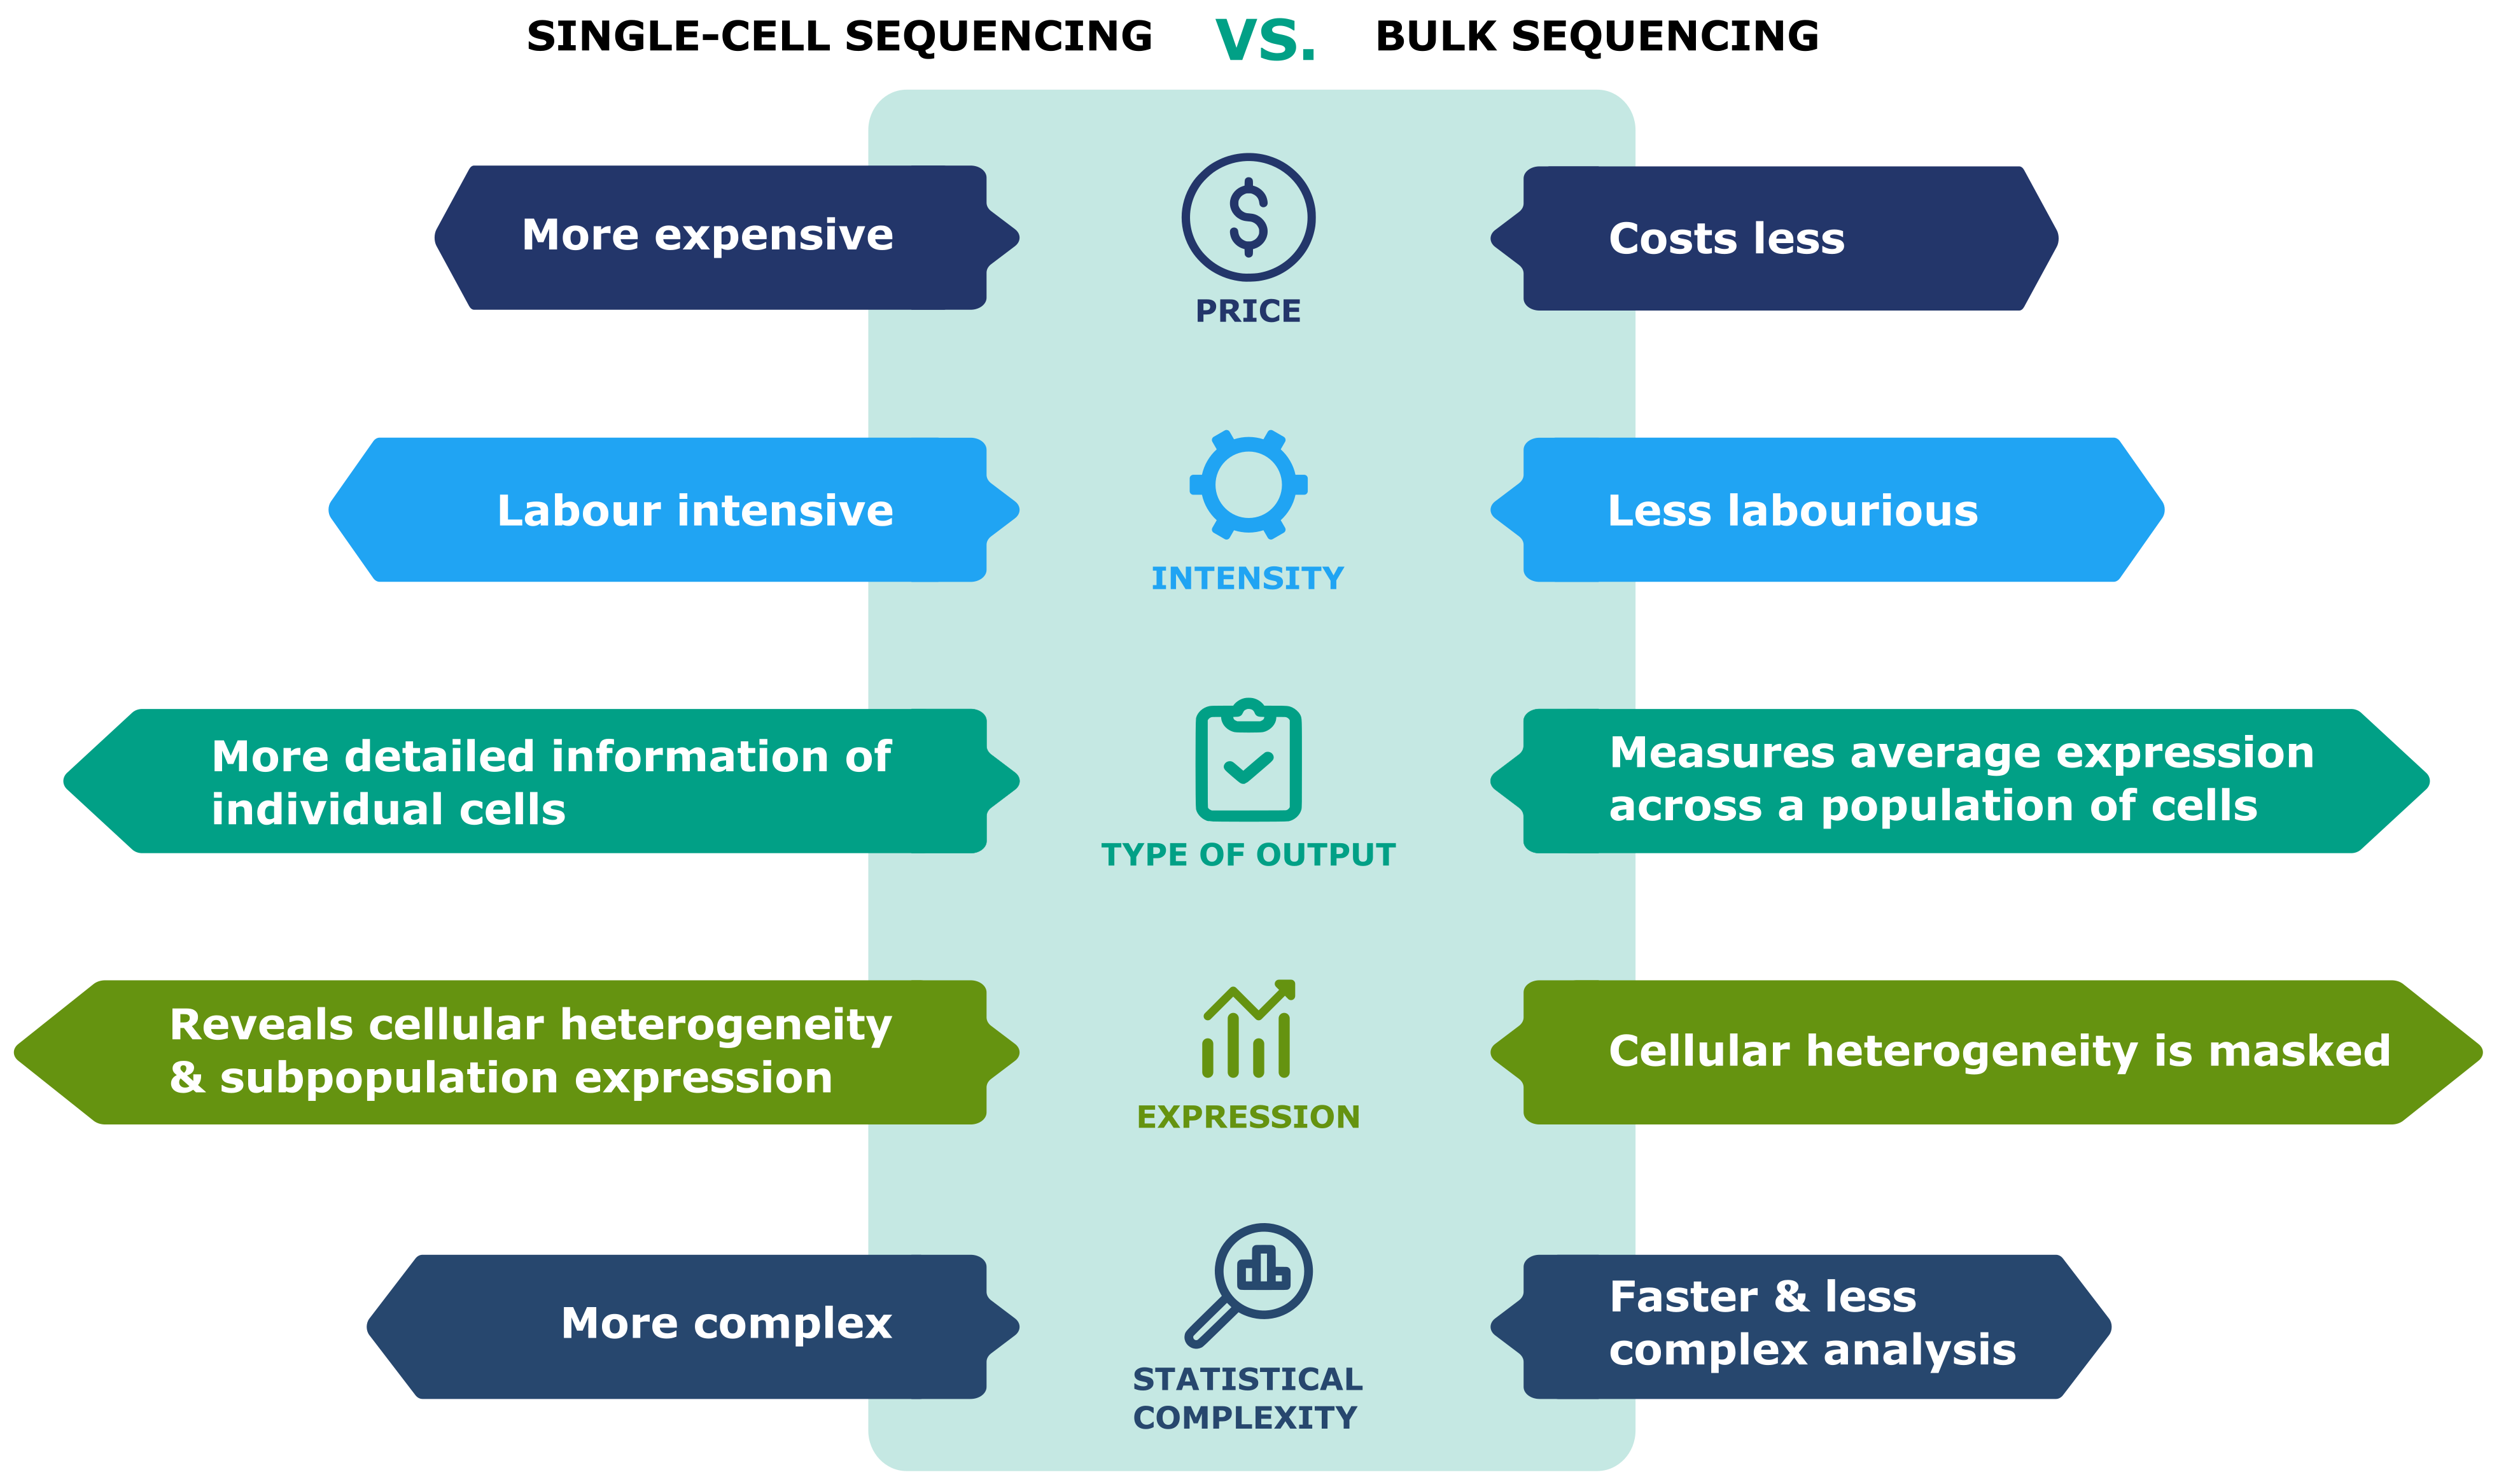
\includegraphics[width=\textwidth]{bulk_vs_sc_01.png}
  \end{figure}
  \end{columns}
\end{frame}

\subsection{细胞异质性}
\begin{frame}
  \frametitle{导言 | 细胞异质性 | 简介}
  \begin{block}{细胞异质性(Heterogeneity)}
    多细胞生物个体由多种形态功能不同的细胞组成;多种类型细胞有序地结合在一起,形成了组织和器官。细胞的异质性是一个普遍存在的生物学现象。\\
    研究细胞异质性,是一个单细胞层面的范畴;单细胞间的异质性存在于DNA、RNA、蛋白质等各个层面。
  \end{block}
  \begin{figure}
    \centering
    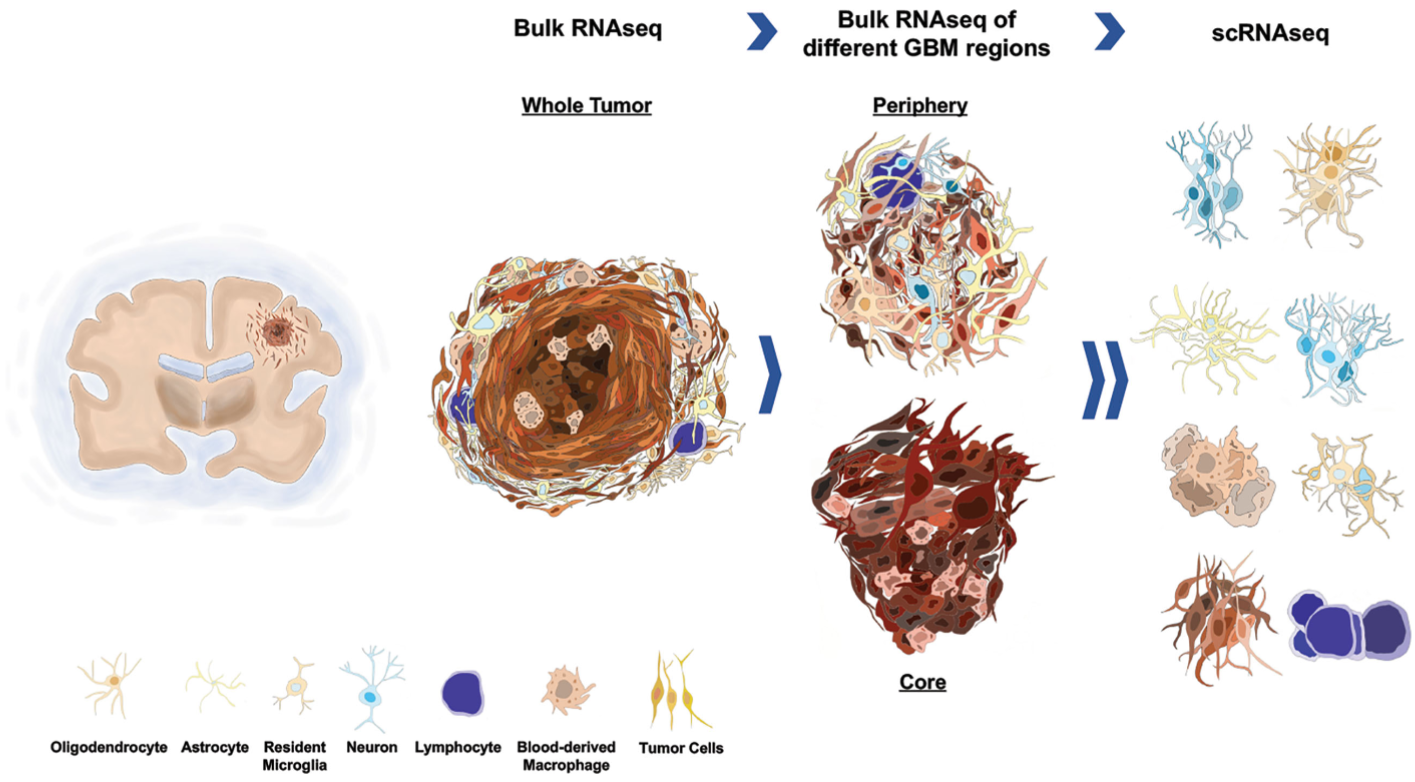
\includegraphics[width=0.7\textwidth]{cell_het.png}
  \end{figure}
\end{frame}
\begin{frame}
  \frametitle{导言 | 肿瘤异质性 | 简介}
  \begin{block}{肿瘤异质性(Tumor heterogeneity)}
    同一种恶性肿瘤在不同患者个体间(肿瘤间异质性,\textbf{Inter}tumor heterogeneity)或者同一患者体内不同部位肿瘤细胞间(肿瘤内异质性,\textbf{Intra}tumor heterogeneity)从基因型到表型上存在的差异。
  \end{block}
  \begin{figure}
    \centering
    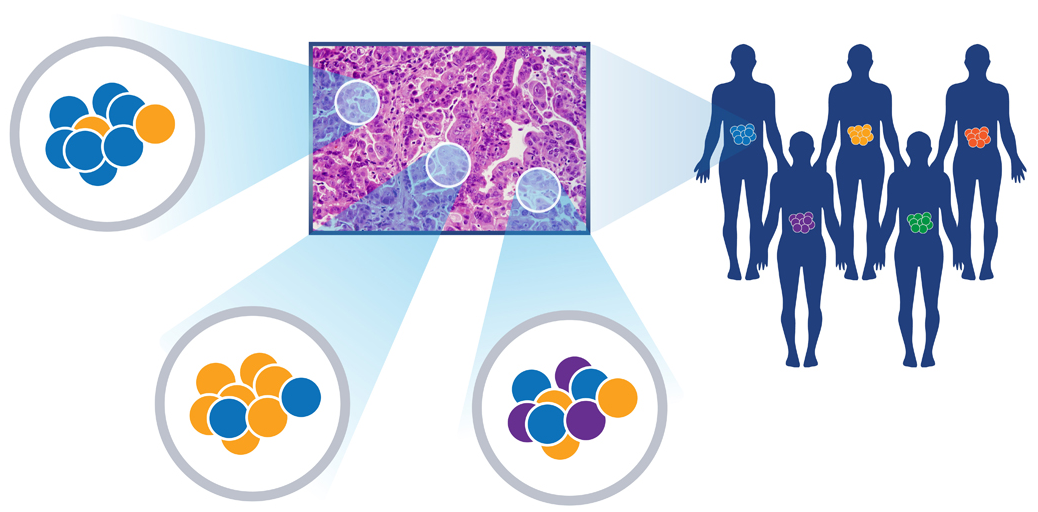
\includegraphics[width=0.8\textwidth]{tumor_het_02.png}
  \end{figure}
\end{frame}
\begin{frame}
  \frametitle{导言 | 肿瘤微环境 | 简介}
  \begin{block}{肿瘤微环境(Tumor microenvironment)}
    肿瘤细胞存在的周围微环境,包括周围的血管、免疫细胞、成纤维细胞、各种信号分子和细胞外基质(ECM)等。 肿瘤微环境有助于肿瘤异质性的形成。
  \end{block}
  \vspace{-0.3em}
  \pause
  \begin{columns}
    \column{0.45\textwidth}
  \begin{block}{肿瘤免疫微环境}
    肿瘤可能被多种免疫相关成分浸润,包括细胞因子/趋化因子、细胞毒性活性或免疫抑制因子。这种免疫异质性在几乎所有实体瘤中普遍存在,并且随着肿瘤的发展以及治疗干预而发生时空变化。
  \end{block}
    \column{0.6\textwidth}
  \begin{figure}
    \centering
    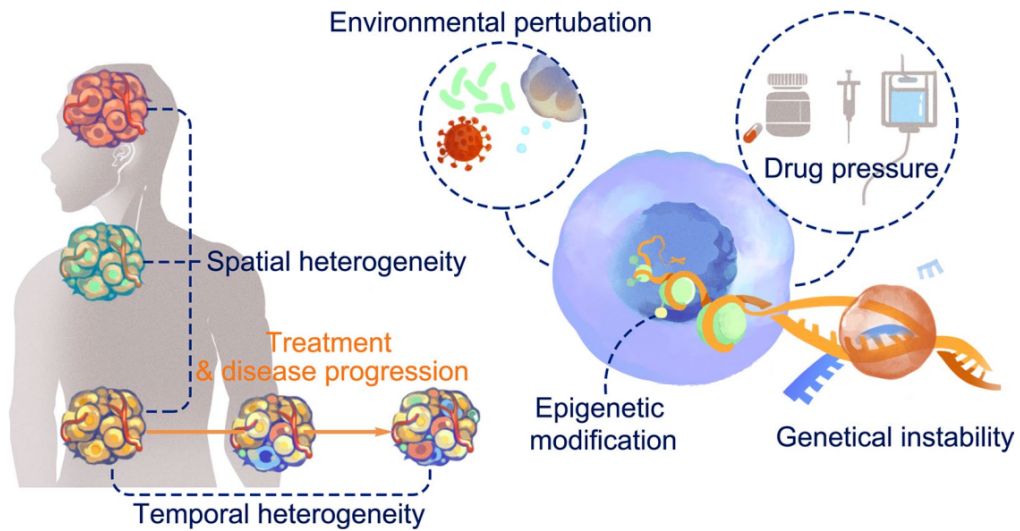
\includegraphics[width=\textwidth]{tumor_imm_het.png}
  \end{figure}
  \end{columns}
\end{frame}

\subsection{单细胞测序}
\begin{frame}
  \frametitle{导言 | 单细胞测序 | 简介}
  \begin{block}{单细胞测序(Single cell sequencing)}
    采取优化的NGS技术检测单细胞的序列,可以获得特定微环境下的细胞序列差异以方便研究其功能差异等。
    \begin{itemize}
      \item DNA测序:了解例如在癌症中的小范围细胞的变异
      \item RNA测序:了解和鉴别不同的细胞类型与其表达的基因
    \end{itemize}
  \end{block}
  \begin{figure}
    \centering
    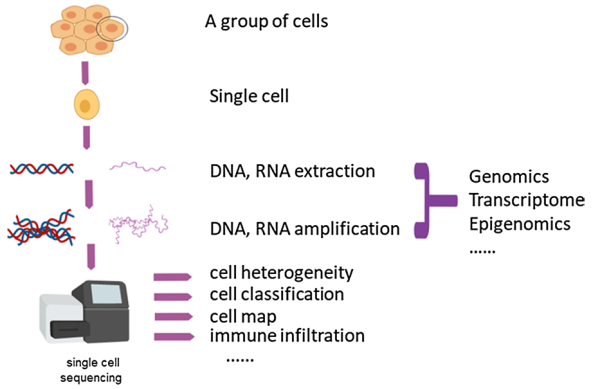
\includegraphics[width=0.48\textwidth]{sc_seq_03.png}
    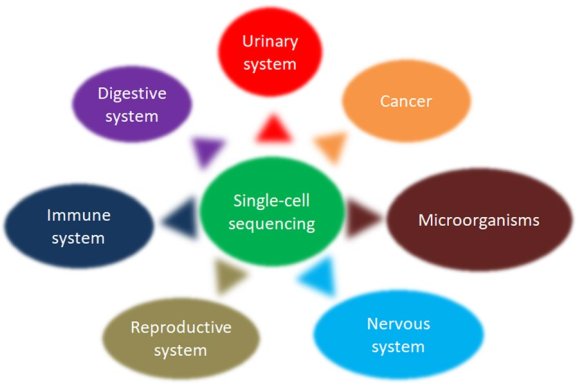
\includegraphics[width=0.48\textwidth]{sc_seq_04.png}
  \end{figure}
\end{frame}
\begin{frame}
  \frametitle{导言 | 单细胞测序 | 技术}
  \begin{figure}
    \centering
    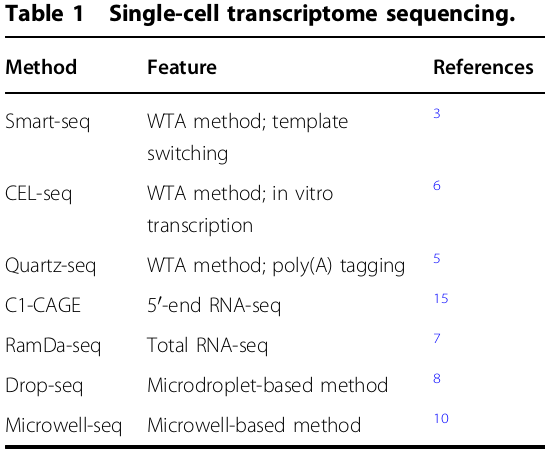
\includegraphics[width=0.36\textwidth]{sc_seq_RNA.png}\hspace{0.5em}
    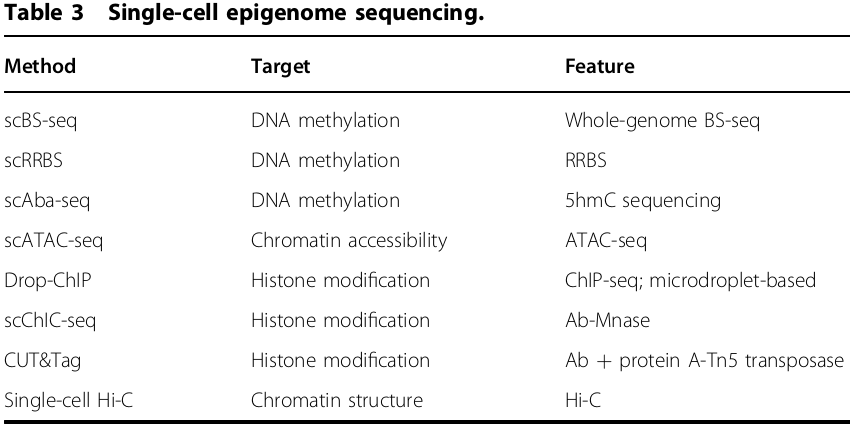
\includegraphics[width=0.6\textwidth]{sc_seq_EPI.png}\\
    \vspace{1em}
    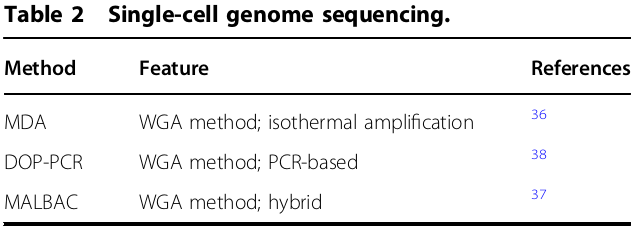
\includegraphics[width=0.45\textwidth]{sc_seq_DNA.png}\hspace{1em}
    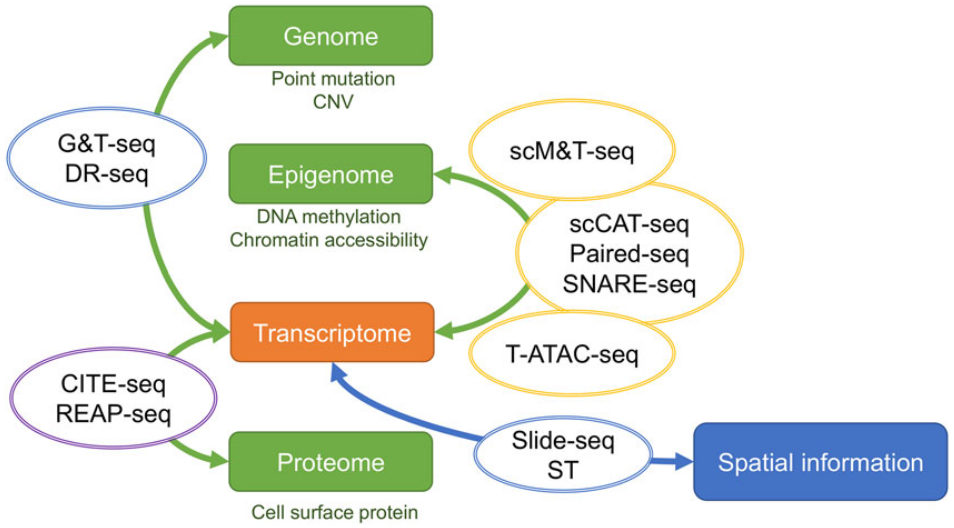
\includegraphics[width=0.5\textwidth]{sc_seq_Multi.png}
  \end{figure}
\end{frame}


\section{单细胞基因组学}
\subsection{应用案例}
\begin{frame}
  \frametitle{scDNA | 应用 | 概述}
  \begin{columns}
    \column{0.5\textwidth}
  \begin{figure}
    \centering
    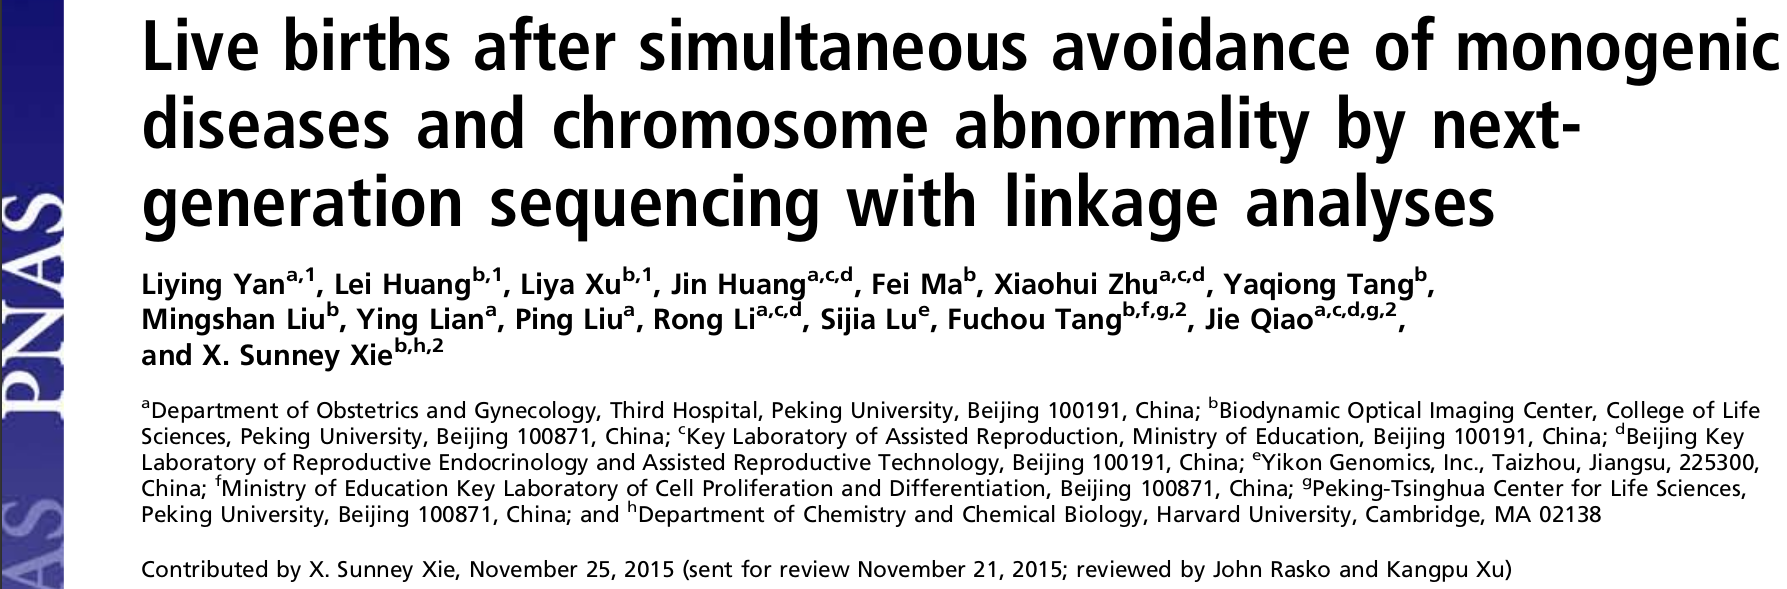
\includegraphics[width=\textwidth]{scDNA_PNAS.png}\\
  \begin{itemize}
    \item 临床应用:胚胎植入前遗传诊断
    \item Liying Yan, et al. \textit{PNAS}, 2015
    \item 北京大学
  \end{itemize}
  \end{figure}
    \column{0.5\textwidth}
  \begin{figure}
    \centering
    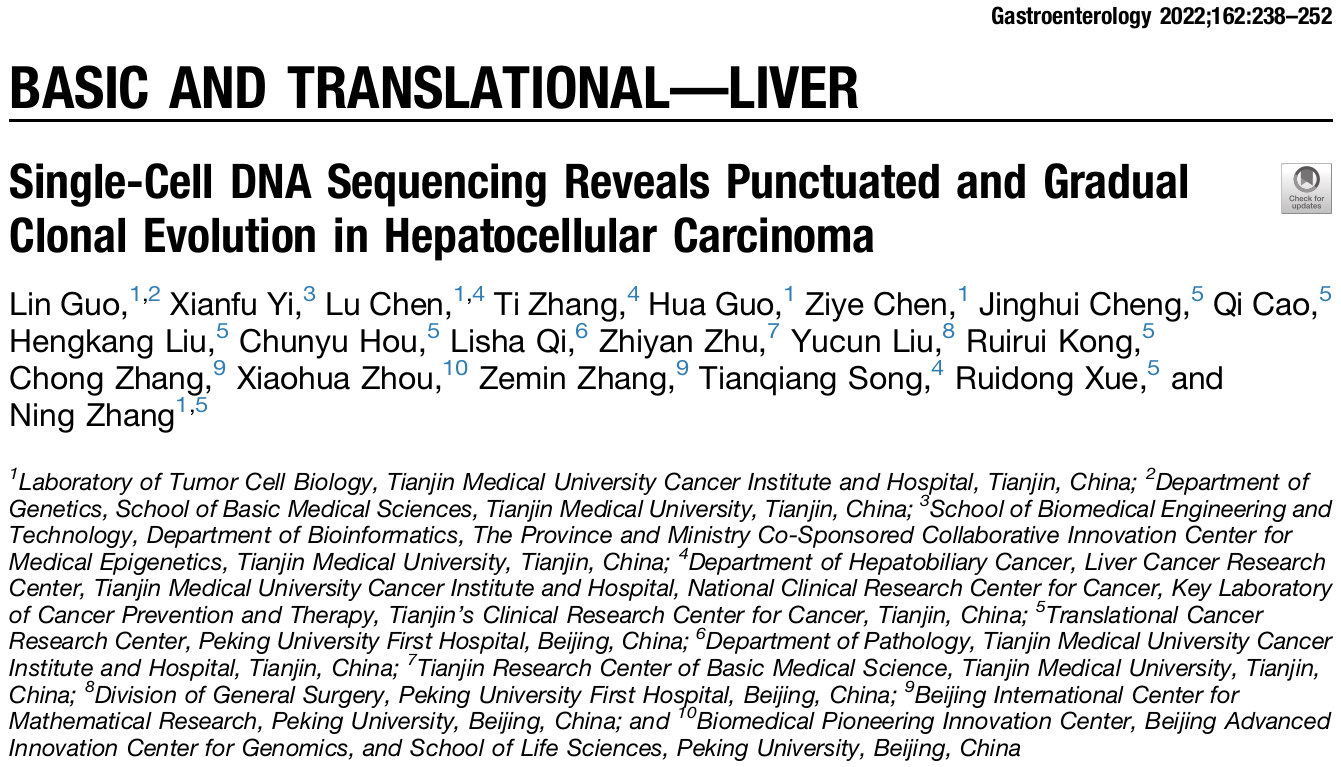
\includegraphics[width=\textwidth]{scDNA_Gastro.png}\\
  \begin{itemize}
    \item 基础研究:肝细胞CNA的双相演化模式
    \item Lin Guo, et al. \textit{Gastro}, 2022
    \item 北京大学 \& 天津医科大学
  \end{itemize}
  \end{figure}
  \end{columns}
\end{frame}
\begin{frame}
  \frametitle{scDNA | 应用 | 胚胎诊断}
  \begin{columns}
    \column{0.7\textwidth}
    \begin{block}{首例MALBAC胚胎全基因组扩增测序试管婴儿}
2014年9月19日,世界首例经MALBAC基因组扩增高通量测序同时筛查单基因遗传病和染色体异常的试管婴儿,在北京大学第三医院诞生,这标志着我国\alert{胚胎植入前遗传诊断技术}跻身世界领先地位。
      \begin{itemize}
        \item 多学科交叉合作的结果
        \item 将基础研究成果成功应用于临床的重要实例
      \end{itemize}
    \end{block}
    \column{0.25\textwidth}
  \begin{figure}
    \centering
    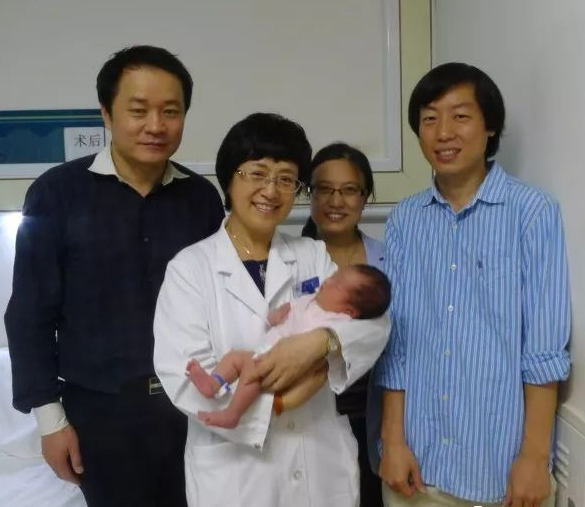
\includegraphics[width=\textwidth]{scDNA_baby.png}\\
    (左起)\\谢晓亮\\乔杰\\闫丽盈\\汤富酬
  \end{figure}
  \end{columns}
\end{frame}
\begin{frame}
  \frametitle{scDNA | 应用 | 胚胎诊断与单细胞}
  \begin{block}{单细胞应用}
在卵母细胞成熟过程中,会产生一个第一极体(含二倍体基因组信息)和一个第二极体(含单倍体基因组信息)作为卵细胞减数分裂的副产物。通过对两个极体细胞进行高通量测序,就能推算出卵细胞本身单倍体是否异常,从而监控早期胚胎是否健康。
  \end{block}
  \begin{block}{胚胎植入前遗传诊断筛查}
      新方法(从刚刚受精的卵细胞上抽取两个被废弃的极体细胞)vs. 传统方法(抽取8细胞期胚胎中的一个细胞):
        \begin{enumerate}
          \item 降低了损伤胚胎的风险
          \item 将植入前诊断的时间窗口从1天增加到2-3天
        \end{enumerate}
  \end{block}
\end{frame}
\begin{frame}
  \frametitle{scDNA | 应用 | 胚胎遗传诊断}
  \begin{block}{遗传病}
    \begin{itemize}
      \item 婴儿的父亲患有遗传性多发性骨软骨瘤(单基因显性遗传病);母亲正常
      \item 由一个基因发生单碱基杂合缺失导致,两人的后代会有50\%的几率患病
    \end{itemize}
  \end{block}
  \vspace{-0.5em}
  \begin{columns}
    \column{0.48\textwidth}
  \begin{figure}
    \centering
    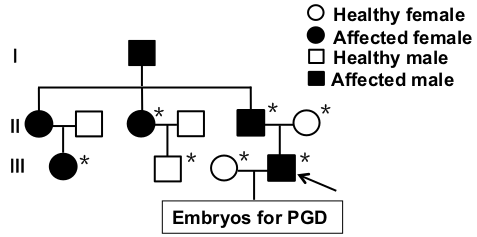
\includegraphics[width=0.85\textwidth]{scDNA_baby_A.png}\\ \vspace{0.3em}
    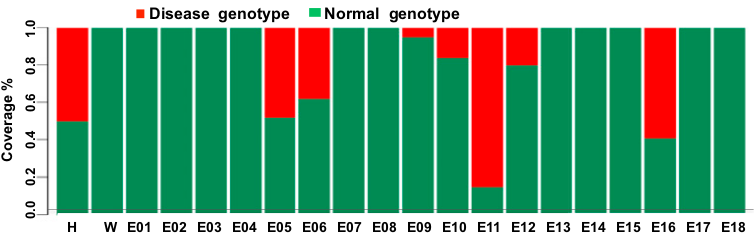
\includegraphics[width=\textwidth]{scDNA_baby_B.png}
  \end{figure}
    \column{0.53\textwidth}
  \begin{figure}
    \centering
    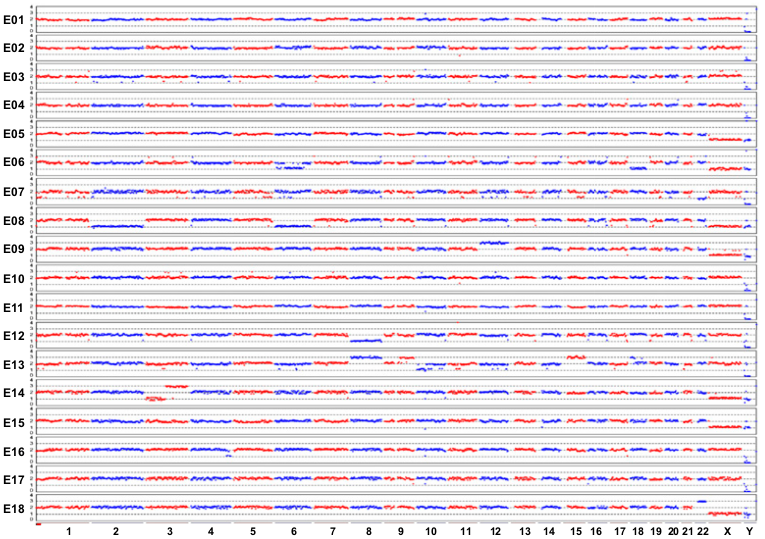
\includegraphics[width=\textwidth]{scDNA_baby_C.png}
  \end{figure}
  \end{columns}
\end{frame}
\begin{frame}
  \frametitle{scDNA | 应用 | 肿瘤演化}
  \begin{block}{研究背景}
    \begin{itemize}
      \item 肿瘤异质性是肝细胞癌(HCC)耐药、复发和预后差的重要原因之一
      \item 基因组不稳定性引起的拷贝数变异(CNA)是肿瘤异质性产生的主要来源
      \item 肝癌的CNA积累遵循渐进演化(GCNE)还是间断演化(PCNE)仍缺乏探究
    \end{itemize}
  \end{block}
  \begin{block}{研究成果}
    \begin{itemize}
      \item 首次提出了肝癌的间断和渐进的双相演化模式(DPCNE)
      \item 揭示了肝癌中双相演化模式与肿瘤内异质性以及预后的关系
    \end{itemize}
  \end{block}
\end{frame}
\begin{frame}
  \frametitle{scDNA | 应用 | 肿瘤演化模型}
  \begin{block}{DPCNE}
    肿瘤染色体不稳定的初始阶段,CNA会高速率累积,短时间内获得大量CNA,呈现间断式演化,随后是一个明显的渐进演化阶段,CNA数目继续积累。
  \end{block}
  \begin{figure}
    \centering
    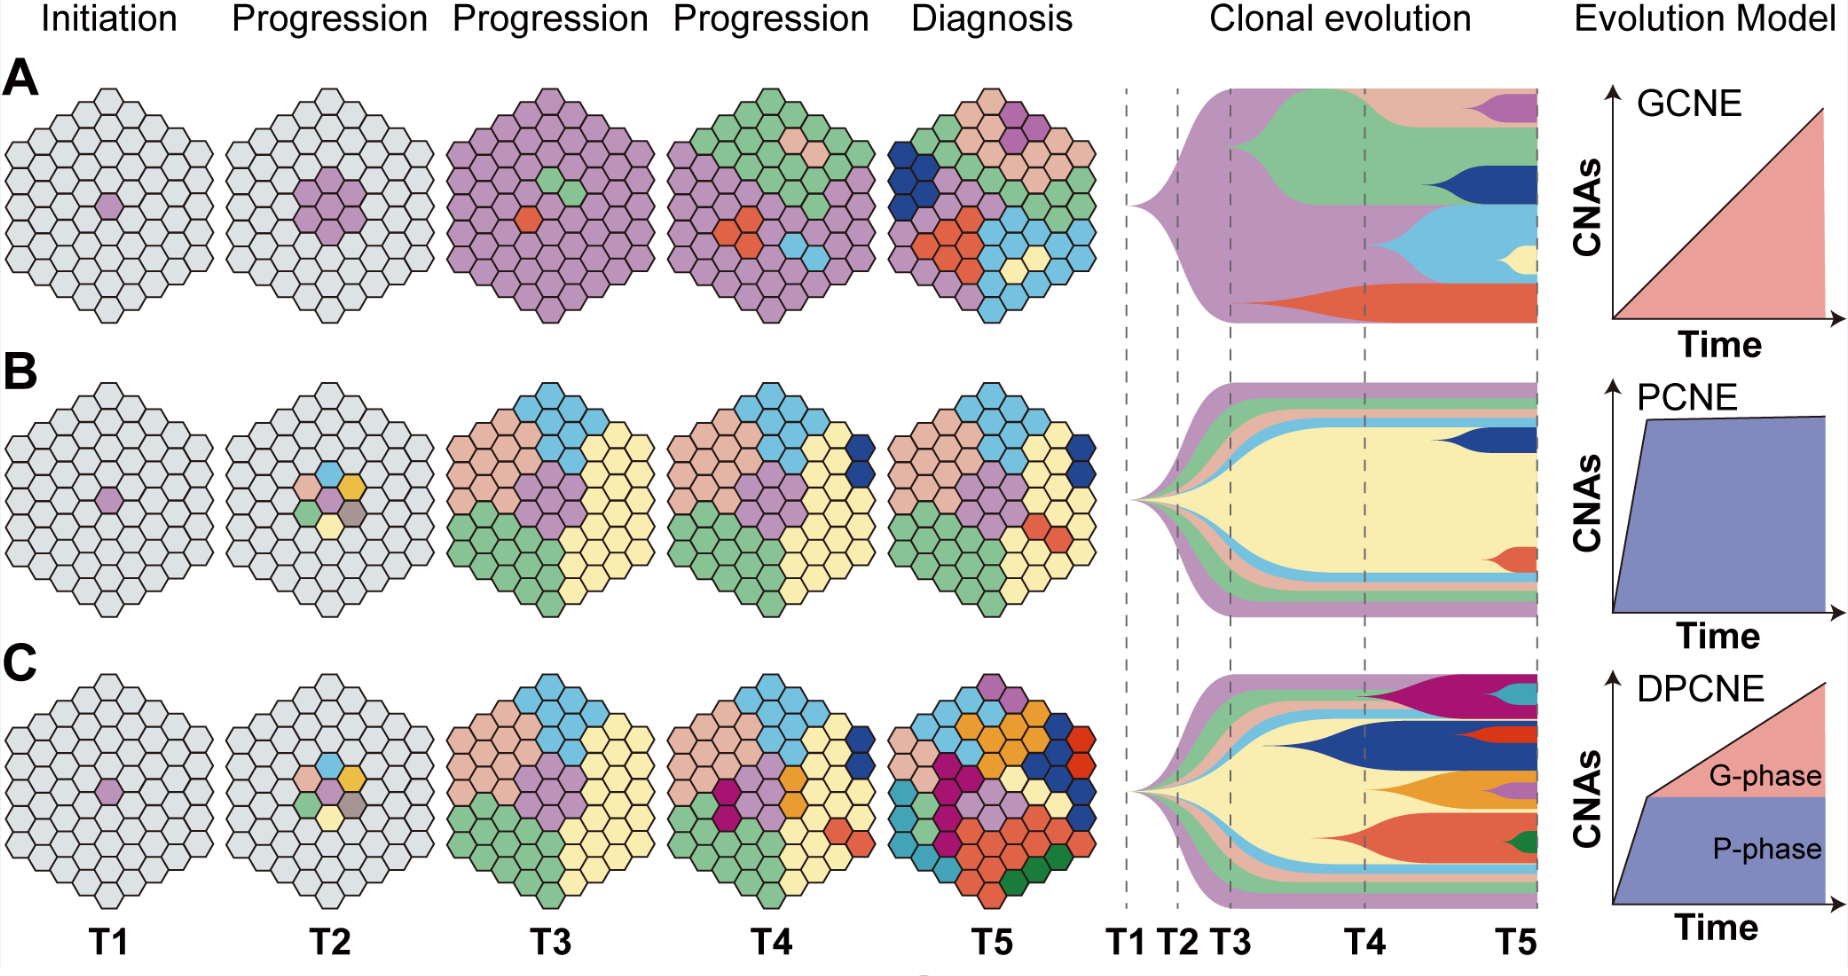
\includegraphics[width=0.9\textwidth]{scDNA_CNA_model.png}
  \end{figure}
\end{frame}

\subsection{实验原理}
\begin{frame}
  \frametitle{scDNA | 简介}
  \begin{block}{单细胞全基因组测序}
在单细胞水平对全基因组进行扩增与测序的一项新技术;将分离的单个细胞的微量全基因组DNA进行扩增,获得高覆盖率的完整的基因组后,进行高通量测序,用于揭示细胞群体差异和细胞进化关系。
  \end{block}
  \vspace{-0.5em}
  \pause
  \begin{columns}
    \column{0.4\textwidth}
    \begin{block}{主要步骤}
      \begin{enumerate}
        \item 单细胞获取
        \item 单细胞全基因组扩增
        \item 扩增产物测序及分析
      \end{enumerate}
    \end{block}
    \column{0.6\textwidth}
  \begin{figure}
    \centering
    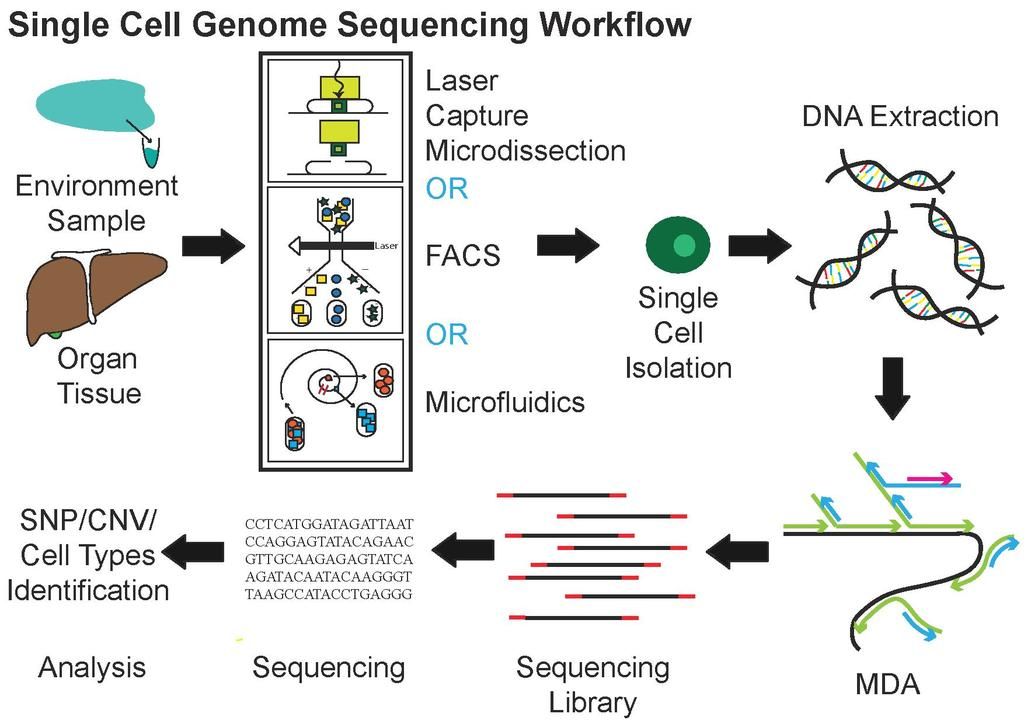
\includegraphics[width=\textwidth]{scDNA_workflow.png}
  \end{figure}
  \end{columns}
\end{frame}
\begin{frame}
  \frametitle{scDNA | 实验原理}
  \begin{block}{单细胞分离技术}
  \begin{figure}
    \centering
    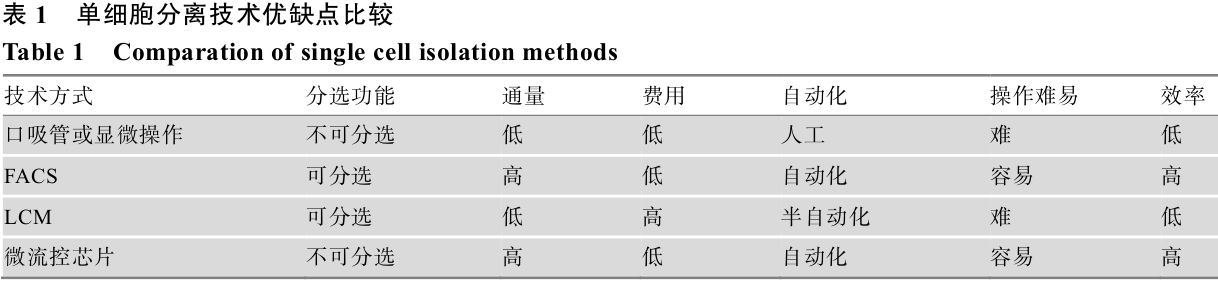
\includegraphics[width=\textwidth]{scDNA_isolation.png}
  \end{figure}
  \end{block}
  \vspace{-0.5em}
  \pause
  \begin{columns}
    \column{0.45\textwidth}
    \begin{block}{单细胞基因组扩增技术}
      \begin{itemize}
        \item 基于PCR扩增
        \item 多重置换扩增(MDA)
        \item 多次退火环状循环扩增(MALBAC)
        \item 线性扩增(LIANTI)
        \item 高通量扩增
      \end{itemize}
    \end{block}
    \column{0.55\textwidth}
  \begin{figure}
    \centering
    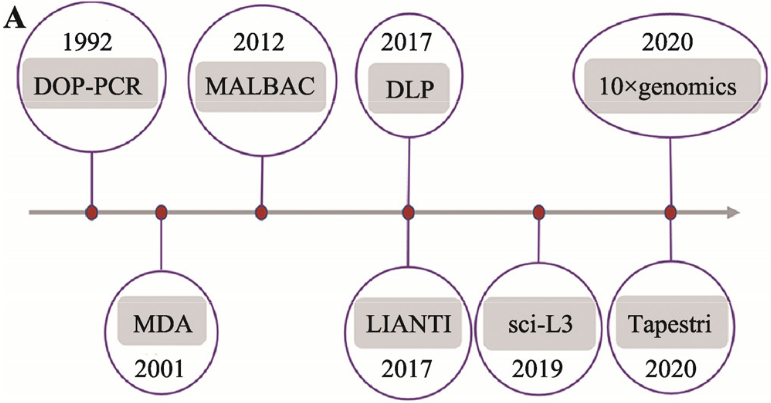
\includegraphics[width=\textwidth]{scDNA_amp.png}
  \end{figure}
  \end{columns}
\end{frame}
\begin{frame}
  \frametitle{scDNA | 应用方向}
  \begin{block}{可以检测单细胞}
    \begin{itemize}
      \item 单碱基突变(single-nucleotide variants,SNV)
      \item 短序列插入/缺失(insertions and deletions,Indel)
      \item \alert{拷贝数变异(copy number variants, CNV)}
      \item 染色体结构变异(structural variation,SV)
    \end{itemize}
  \end{block}
  \begin{figure}
    \centering
    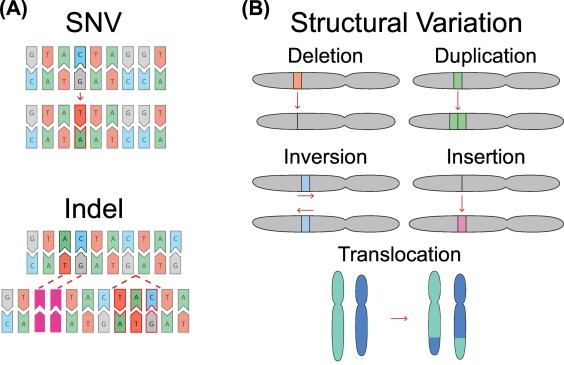
\includegraphics[width=0.55\textwidth]{scDNA_var_02.png}\quad
    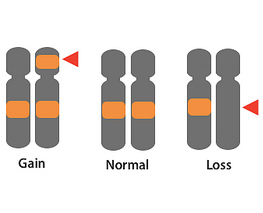
\includegraphics[width=0.4\textwidth]{scDNA_var_09.png}
  \end{figure}
\end{frame}

\subsection{分析策略}
\begin{frame}
  \frametitle{scDNA | CNV | 分析概述}
  \begin{columns}
    \column{0.5\textwidth}
  \begin{figure}
    \centering
    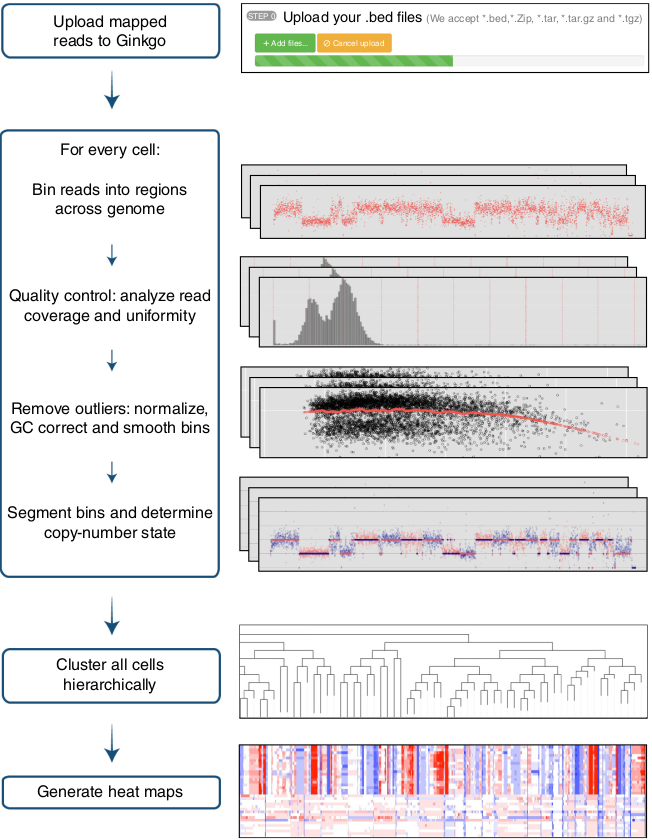
\includegraphics[width=\textwidth]{scDNA_CNA_workflow_02.png}
  \end{figure}
    \column{0.5\textwidth}
  \begin{figure}
    \centering
    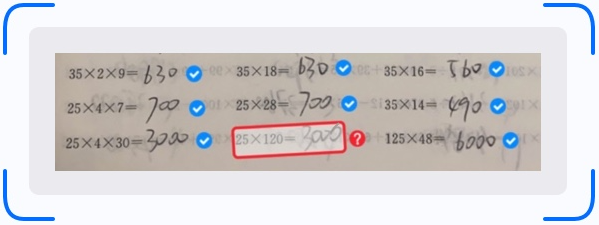
\includegraphics[width=0.8\textwidth]{scDNA_OCR_01.png}\\
    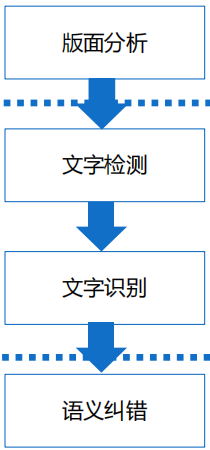
\includegraphics[width=0.3\textwidth]{scDNA_OCR_09.png}\\ \vspace{0.7em}
    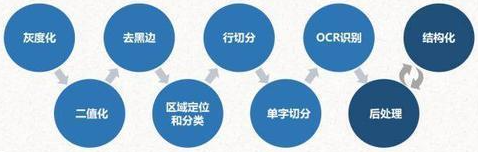
\includegraphics[width=\textwidth]{scDNA_OCR_10.png}
  \end{figure}
  \end{columns}
\end{frame}
\begin{frame}
  \frametitle{scDNA | CNV | 分析步骤}
  \begin{columns}
    \column{0.42\textwidth}
    \begin{enumerate}
      \item Binning
      \item GC correction
      \item Mappability correction
      \item Removal of outlier bins
      \item Removal of outlier cells
      \item Segmentation
      \item Calling the absolute copy numbers
    \end{enumerate}
    \column{0.58\textwidth}
  \begin{figure}
    \centering
    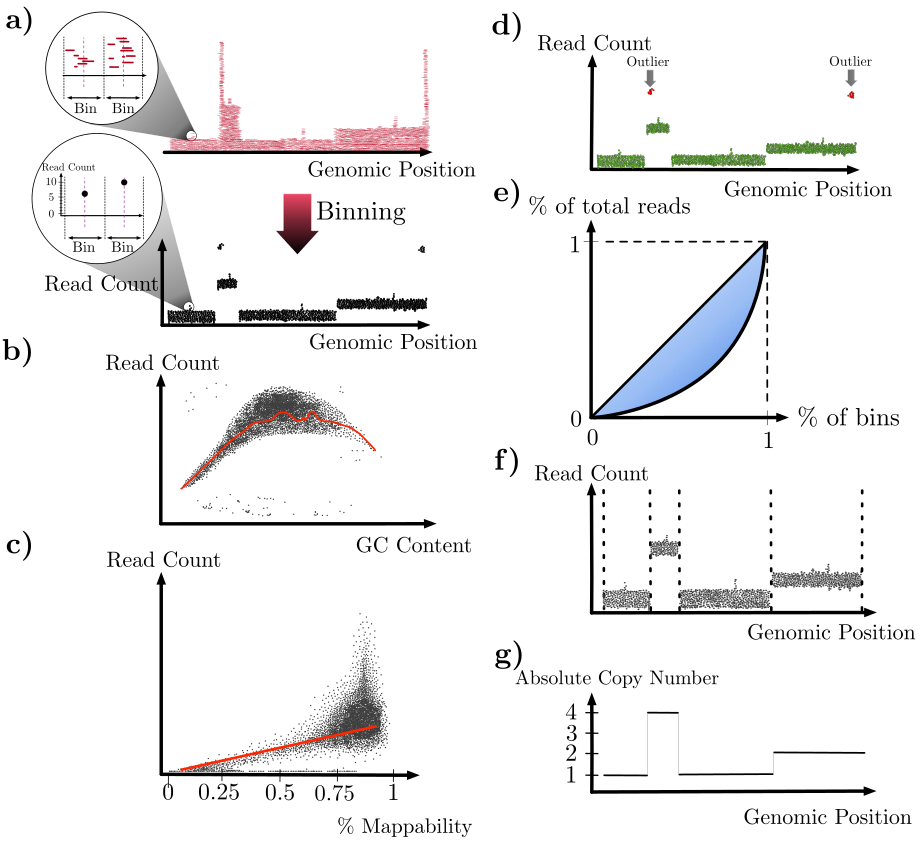
\includegraphics[width=\textwidth]{scDNA_CNA_workflow_03.png}
  \end{figure}
  \end{columns}
\end{frame}
\begin{frame}
  \frametitle{scDNA | CNV | 分析工具}
  \begin{figure}
    \centering
    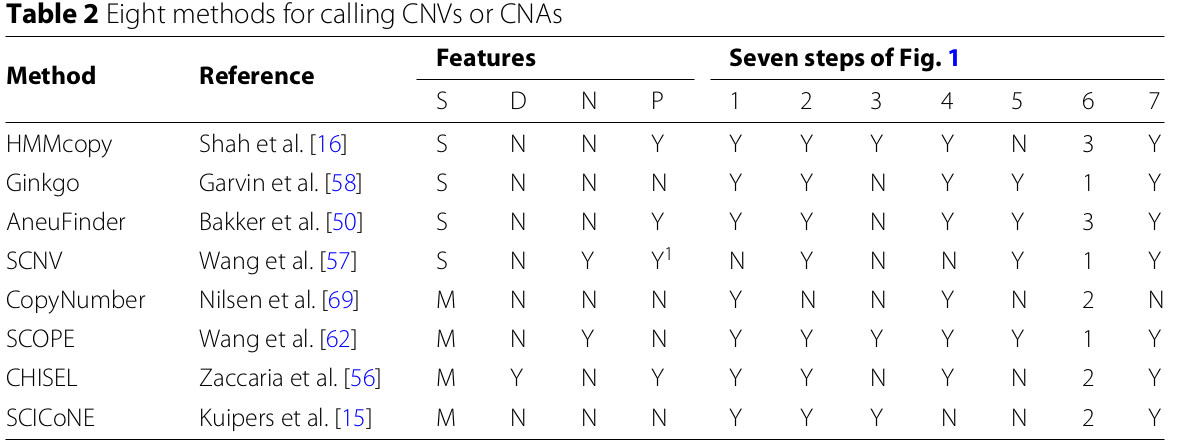
\includegraphics[width=\textwidth]{scDNA_CNA_tools.png}\\ \vspace{1em}
    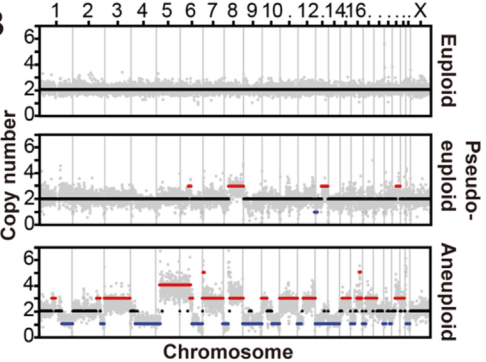
\includegraphics[width=0.28\textwidth]{scDNA_CNA_out_01.png}
    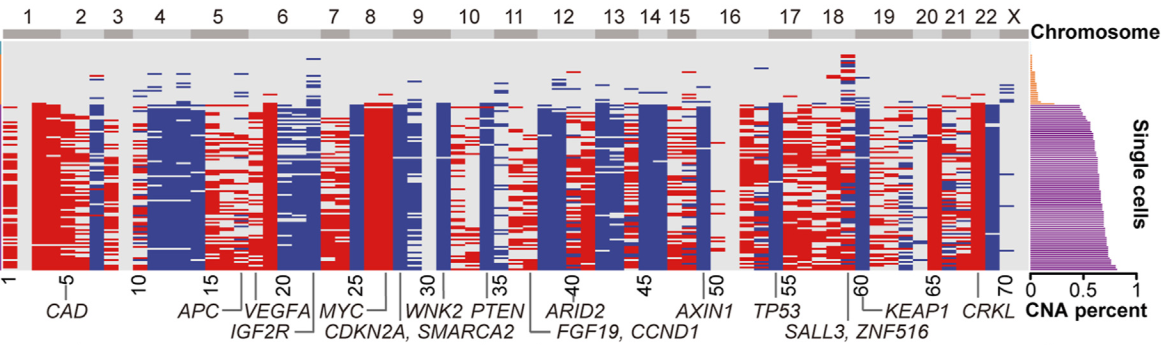
\includegraphics[width=0.7\textwidth]{scDNA_CNA_out_02.png}
  \end{figure}
\end{frame}

\subsection{评刊论号}
\begin{frame}
\frametitle{评书刊号|书籍}
\begin{quotation}[《朱子论定程董学则》]
非圣贤之书, 勿读。无益之文, 勿观。
\end{quotation}
\begin{columns}
  \column{0.55\textwidth}
  \begin{block}{古籍}
    \begin{itemize}
      \item 中华书局
      \item 上海古籍出版社
      \item 岳麓书社
      \item 齐鲁书社
      \item 生活・读书・新知三联书店
    \end{itemize}
  \end{block}
  \column{0.38\textwidth}
  \begin{block}{科技}
    \begin{itemize}
      \item 科学出版社
      \item 机械工业出版社
      \item 人民邮电出版社
      \item 清华大学出版社
      \item 电子工业出版社
    \end{itemize}
  \end{block}
\end{columns}
\end{frame}
\begin{frame}
\frametitle{评书刊号|期刊}
\begin{columns}
  \column{0.45\textwidth}
  \begin{block}{综合性期刊}
    \begin{itemize}
      \item \textit{\textbf{C}ell}
      \item \textit{\textbf{N}ature}
      \item \textit{\textbf{S}cience}
      \item \textit{Nature Communications}
      \item \textit{Science Advances}
      \item \textit{PNAS}
      \item \textit{eLife}
    \end{itemize}
  \end{block}
  \column{0.53\textwidth}
  \begin{block}{生信期刊}
    \begin{itemize}
      \item \textit{Nature Genetics}
      \item \textit{Nature Biotechnology}
      \item \textit{Nature Methods}
      \item \textit{Genome Biology}
      \item \textit{Genome Research}
      \item \textit{Nucleic Acids Research}
      \item \textit{PLoS Computational Biology}
      \item \textit{Bioinformatics}
    \end{itemize}
  \end{block}
\end{columns}
\end{frame}
\begin{frame}
\frametitle{评书刊号|公众号}
  \begin{figure}
    \centering
    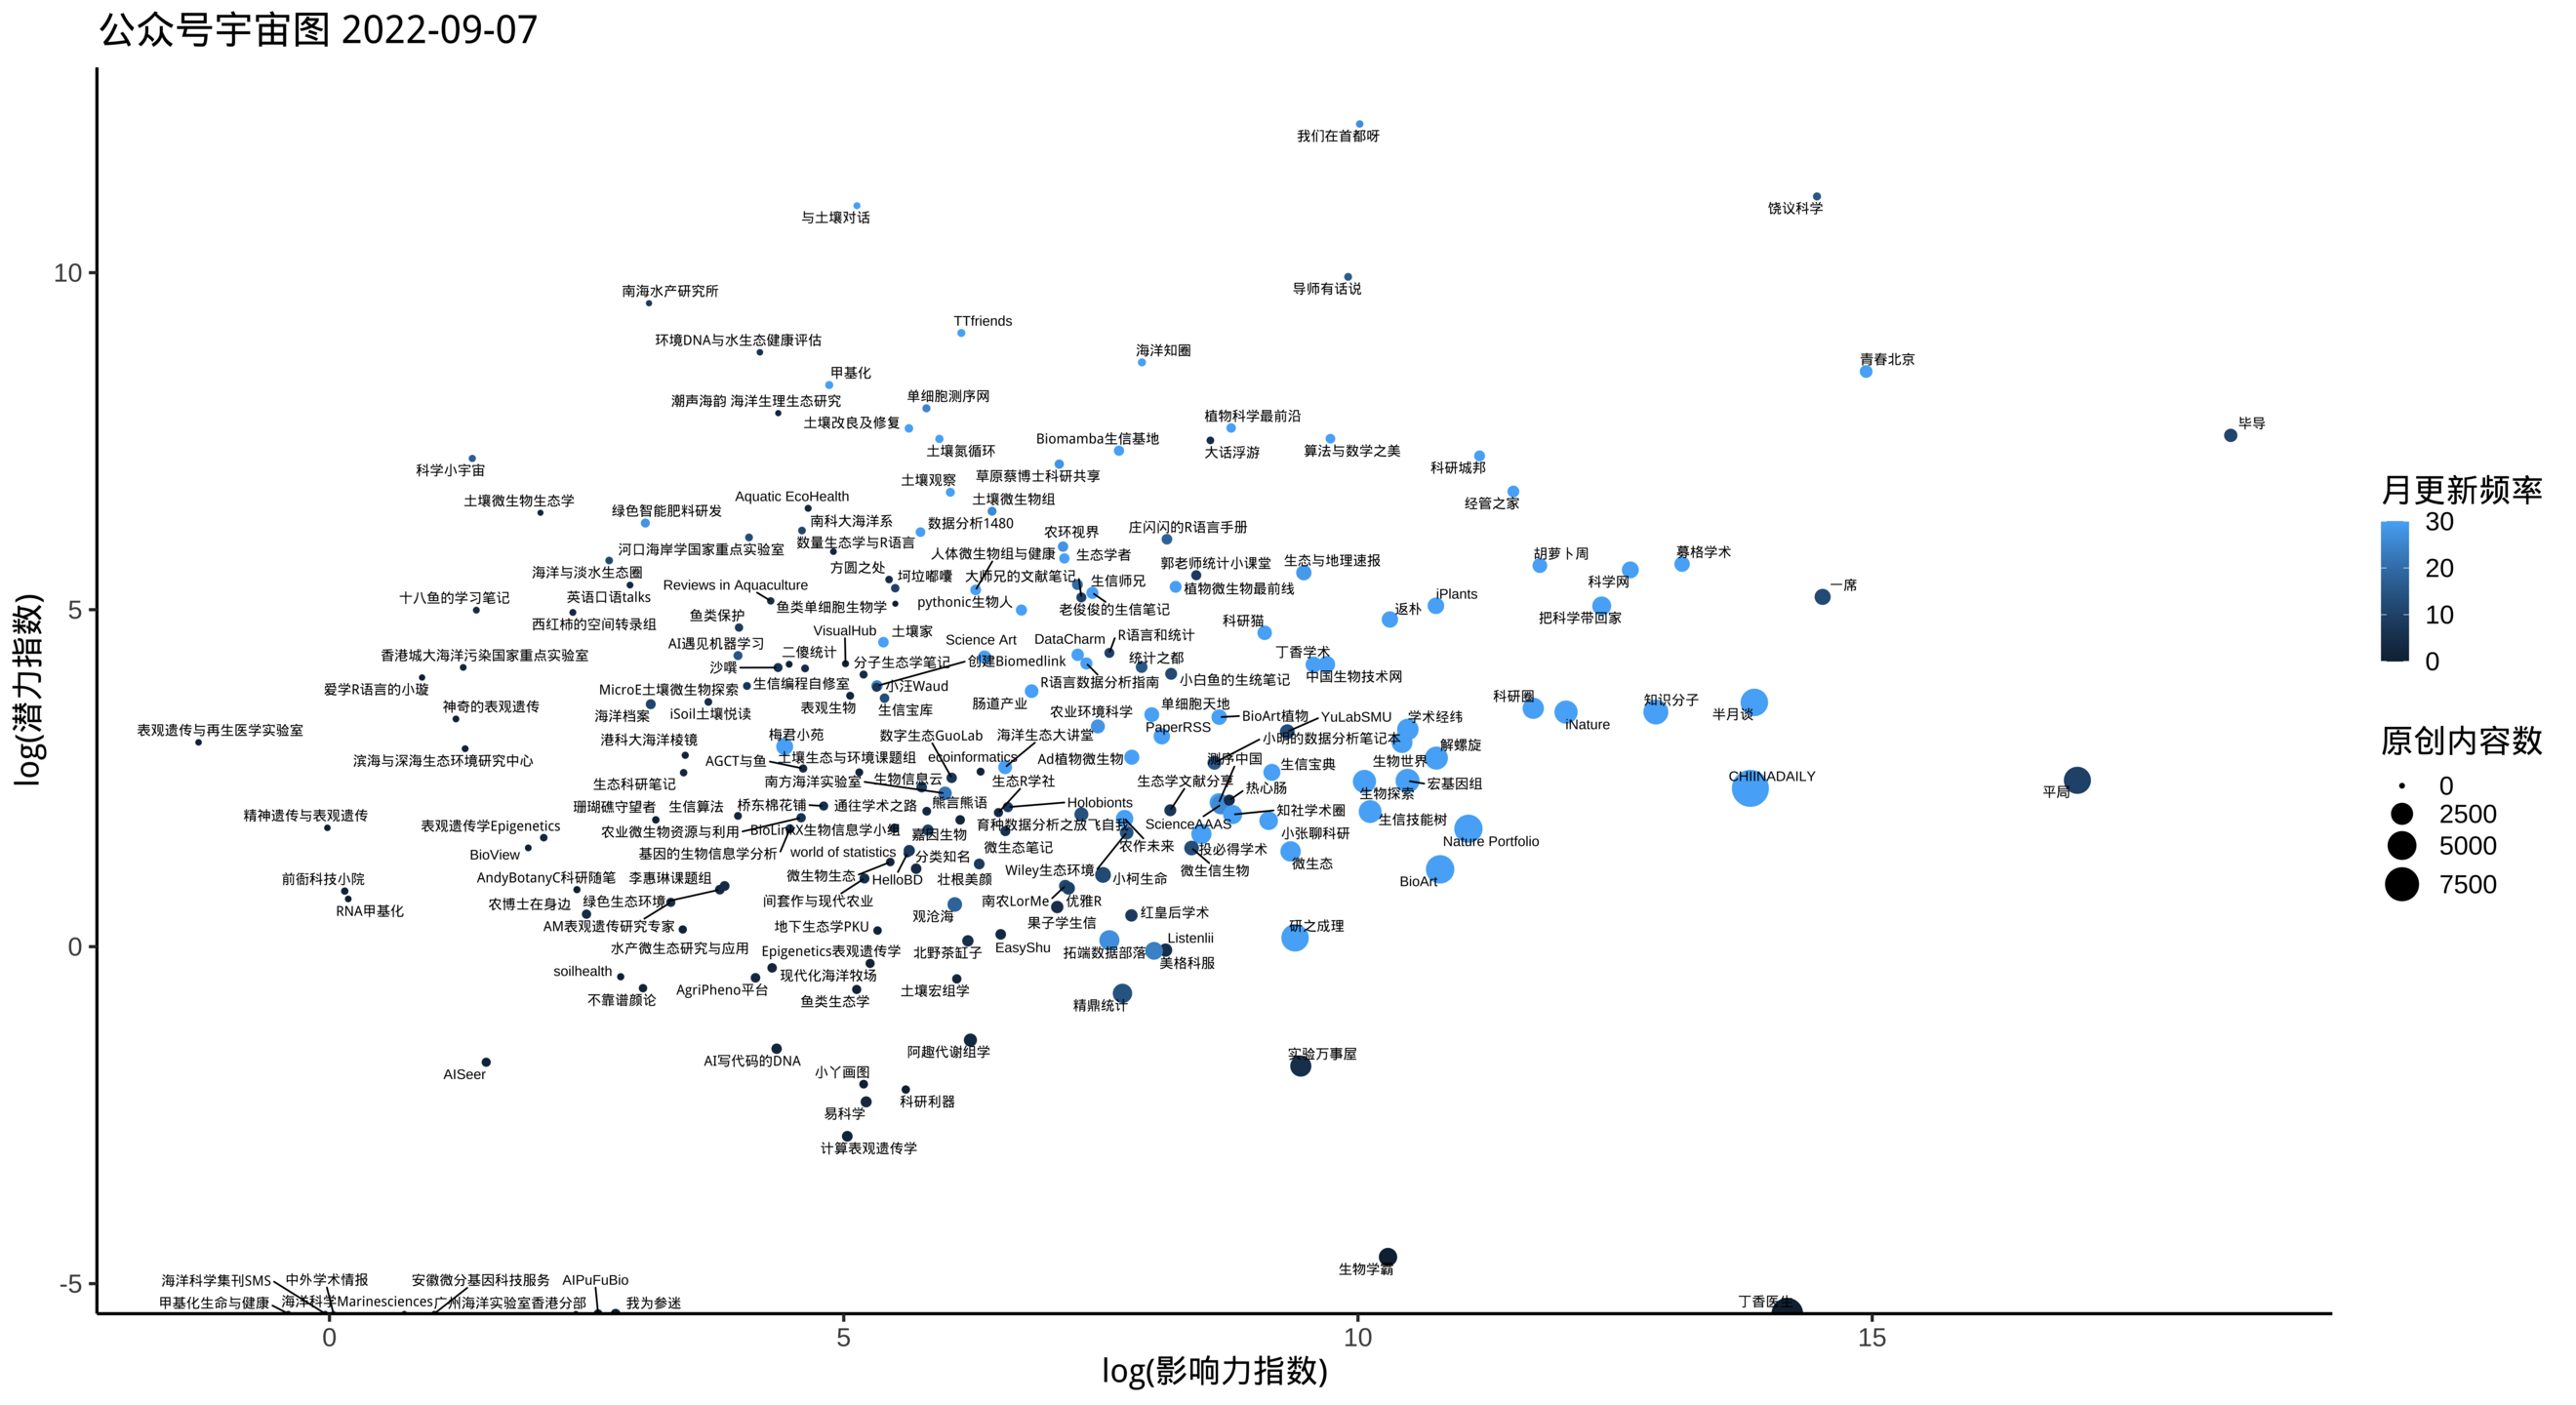
\includegraphics[width=1.05\textwidth]{wechat_02.png}
  \end{figure}
\end{frame}
\begin{frame}
\frametitle{评书刊号|公众号}
  \begin{figure}
    \centering
    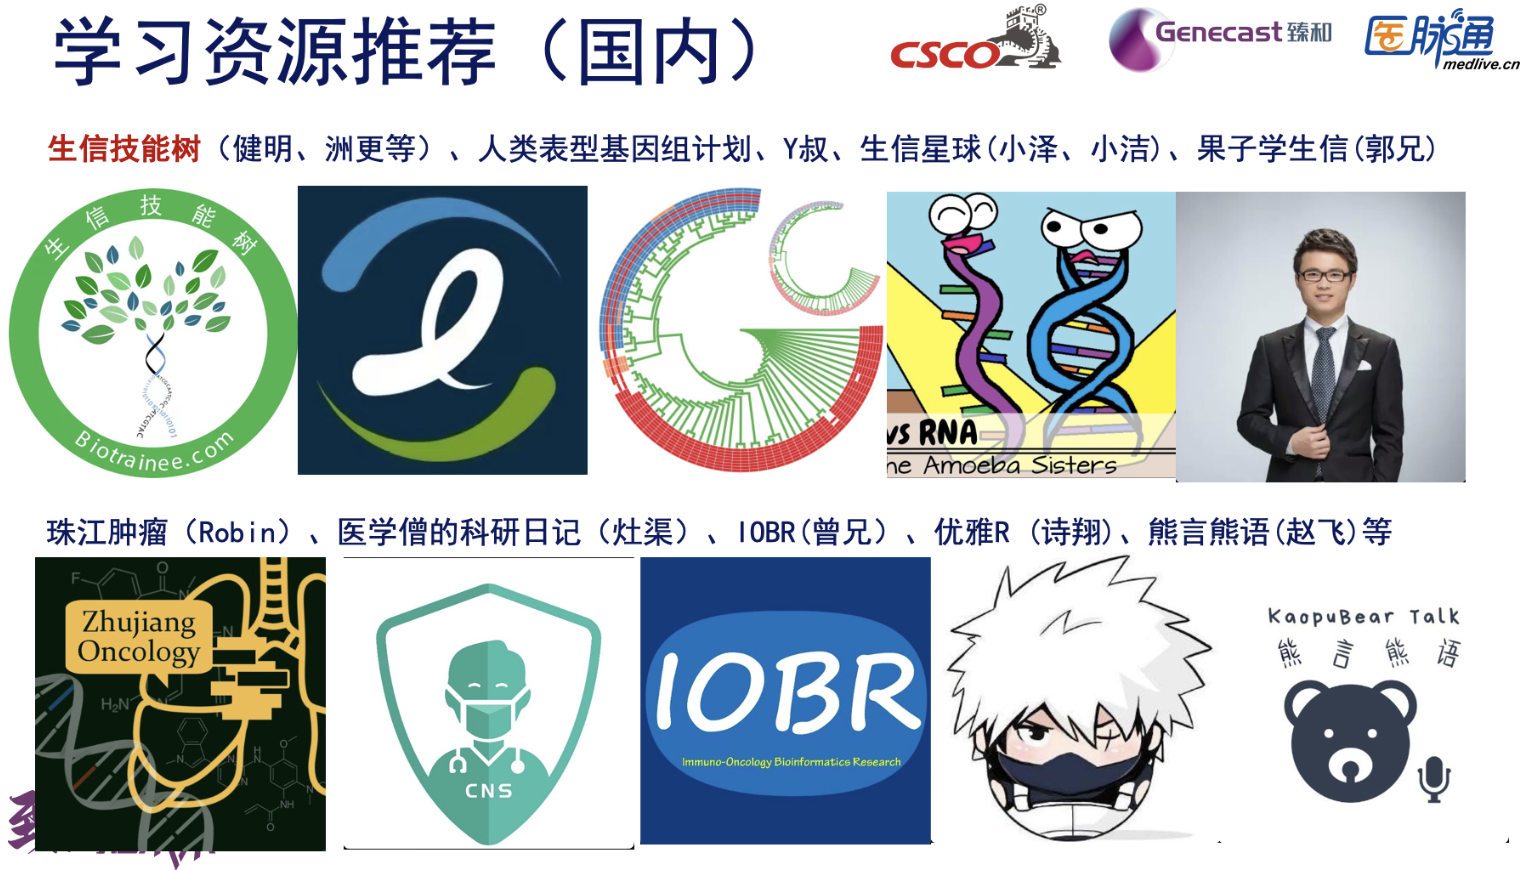
\includegraphics[width=\textwidth]{wechat_01.png}
  \end{figure}
\end{frame}


\section{单细胞转录组学}
\subsection{应用案例}
\begin{frame}
  \frametitle{scRNA | 应用 | 肿瘤}
  \begin{columns}
  \column{0.65\textwidth}
    \begin{block}{肿瘤}
  肿瘤是一个具有高度复杂性的整体,其发生、发展、转移等过程离不开与其所处微环境持续的相互作用。\\
  上皮组织肿瘤由不同来源的复杂且异质的多种细胞类型团块组成,可分为两类:从上皮组织起源癌细胞和\alert{基质细胞}。
  \end{block}
  \column{0.35\textwidth}
    \begin{figure}
    \centering
    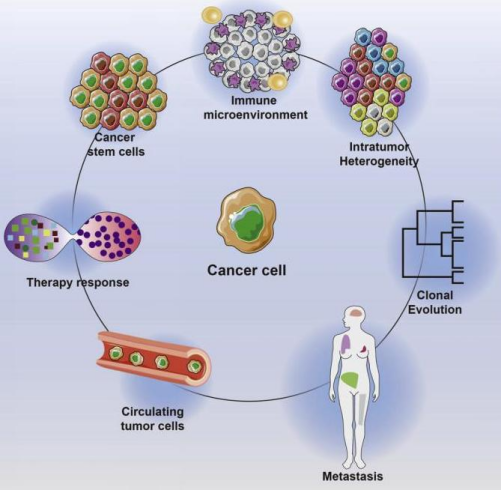
\includegraphics[width=\textwidth]{tumor_01.png}
  \end{figure}
  \end{columns}
    \begin{figure}
    \centering
    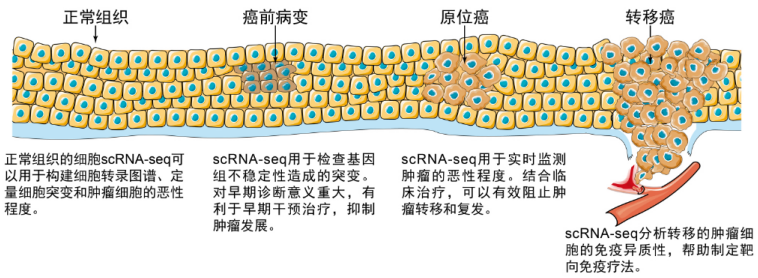
\includegraphics[width=0.8\textwidth]{tumor_02.png}
  \end{figure}
\end{frame}

\begin{frame}
  \frametitle{scRNA | 应用 |  肿瘤微环境}
  \begin{block}{肿瘤微环境(TME, tumor microenvironment)}
  \begin{itemize}
    \item 基质细胞
    \begin{itemize}
      \item 血管生成性血管细胞(AVC)
      \item 癌症相关的成纤维细胞(CAF)
      \item \alert{浸润性免疫细胞(IIC)}:杀伤肿瘤细胞 vs. 促进肿瘤发展
      \begin{itemize}
        \item 肿瘤相关巨噬细胞(TAM)
        \item 肥大细胞
        \item T淋巴细胞
        \item B淋巴细胞
        \item 自然杀伤细胞(NK)
        \item 髓系抑制细胞(MDSC)
        \item ……
      \end{itemize}
    \end{itemize}
    \item 细胞外基质
  \end{itemize}
  \end{block}
\end{frame}

\begin{frame}
  \frametitle{scRNA | 应用 | scRNA与肿瘤免疫微环境}
    \begin{columns}
  \column{0.65\textwidth}
    \begin{block}{scRNA在肿瘤免疫微环境研究中的应用}
    \begin{itemize}
      \item 精确刻画细胞类群及相应的转录特征
      \item 描述微环境内免疫细胞的发育轨迹
      \item 研究肿瘤免疫抑制的分子机制
      \item 分析外界因素对肿瘤免疫产生的影响
      \item 发现临床上新的免疫治疗靶点
      \item 分析不同类型肿瘤患者的生存预后
    \end{itemize}
   \end{block}
  \column{0.4\textwidth}
    \begin{figure}
    \centering
    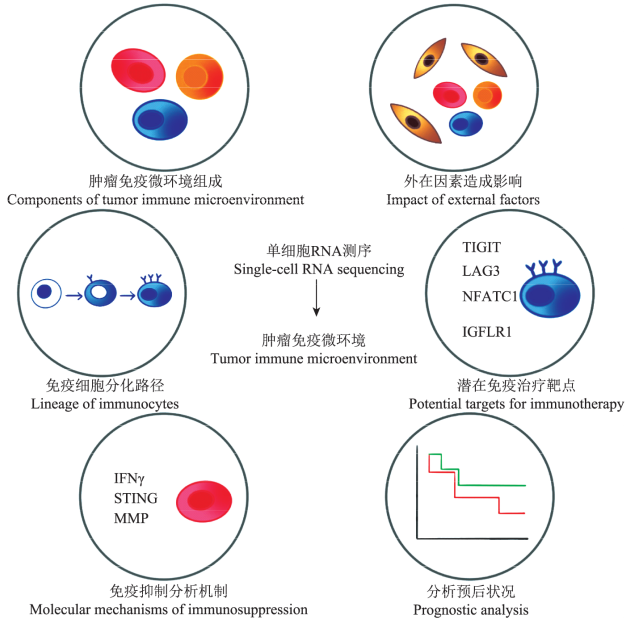
\includegraphics[width=\textwidth]{tumor_scRNA_01.png}
  \end{figure}
  \end{columns}
\end{frame}

\begin{frame}
  \frametitle{scRNA | 应用 | 免疫治疗}
  \begin{block}{免疫治疗(Immunotherapy)}
  通过诱导、增强或抑制免疫反应的疾病治疗方法。
  \begin{itemize}
    \item 激活免疫疗法:引起或增强免疫反应的免疫疗法
    \item 抑制免疫疗法:减少或抑制免疫反应的免疫疗法
  \end{itemize}
  \end{block}
  \pause
  \begin{columns}
  \column{0.45\textwidth}
    \begin{block}{PD-1/PD-L1免疫疗法}
 通过阻断PD-1/PD-L1信号通路,使肿瘤细胞遭受淋巴细胞的免疫袭击从而使癌细胞死亡。具有治疗多种类型肿瘤的潜力,有望实质性地改善患者的总生存期。
  \end{block}
  \column{0.6\textwidth}
     \begin{figure}
    \centering
    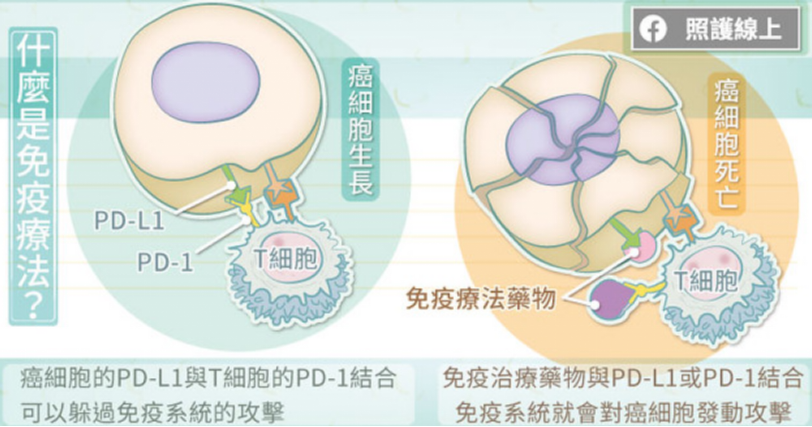
\includegraphics[width=\textwidth]{tumor_PD1_01.png}
  \end{figure}
 \end{columns}
\end{frame}

\begin{frame}
  \frametitle{scRNA | 应用 | 免疫疗法 | 问题}
  \begin{block}{免疫疗法的现状}
  免疫检查点阻断疗法(ICB)已经在非小细胞肺癌(NSCLC)的临床治疗中取得了前所未有的效果。然而对免疫治疗产生显著应答的 NSCLS 患者仍然只是少数。这说明尽管免疫治疗的原理我们都懂,但对于其背后的复杂分子机制,以及同类型癌症患者的肿瘤免疫浸润细胞组分异质性,我们还不够了解。
  \end{block}
   \begin{figure}
    \centering
    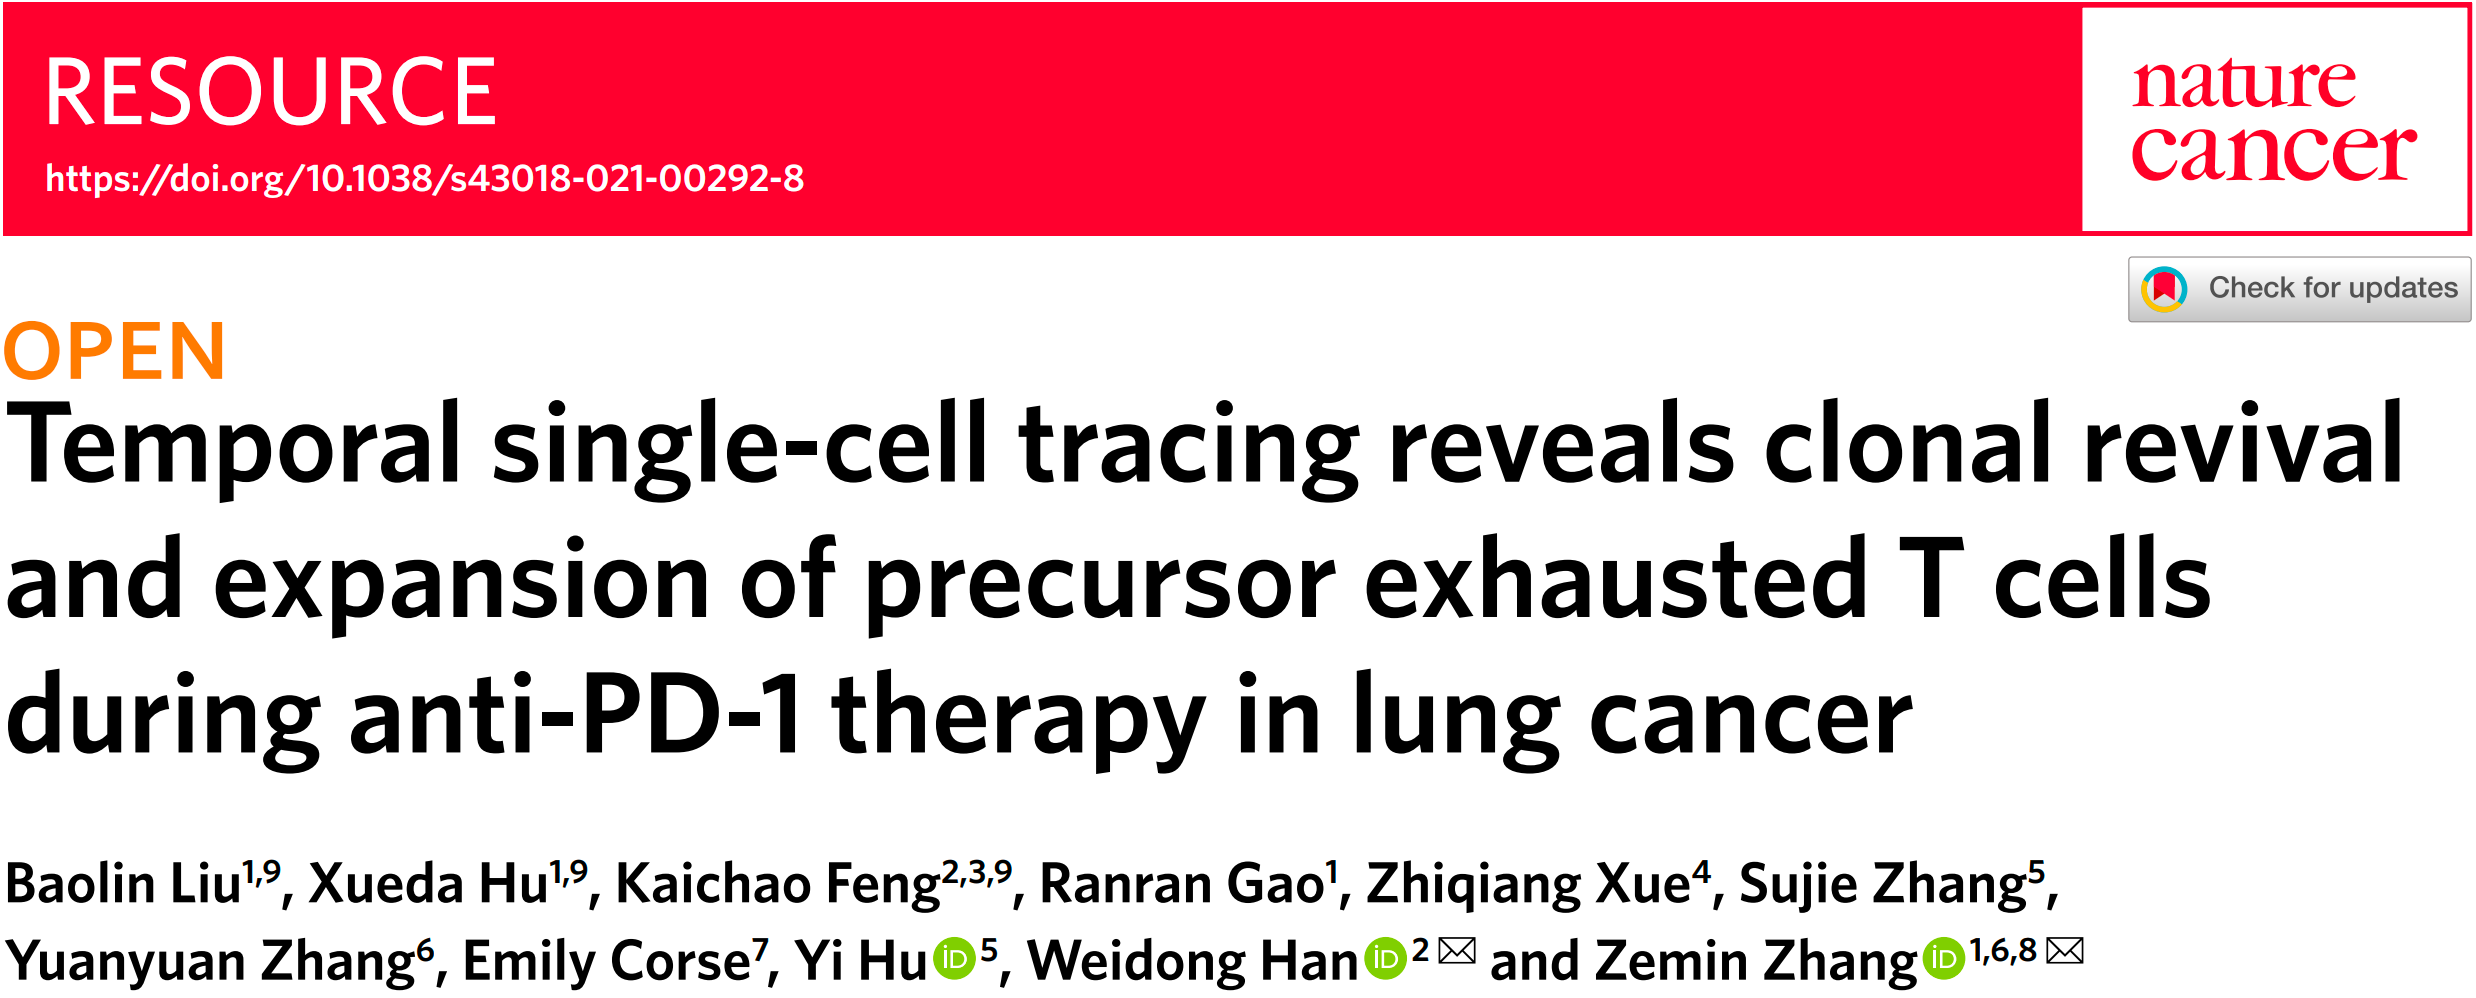
\includegraphics[width=0.9\textwidth]{PD1_NC.png}
  \end{figure}
\end{frame}

\begin{frame}
  \frametitle{scRNA | 应用 | 免疫疗法 | 实验设计}
  \begin{block}{实验设计}
    \begin{itemize}
      \item 36个NSCLC病人,PD1抑制剂治疗(+ 化疗)
      \item 47例肿瘤样本 = 33治疗前 + 9治疗后有效 + 5治疗后无效
      \item scRNA-seq + scTCR-seq
    \end{itemize}
  \end{block}
   \begin{figure}
    \centering
    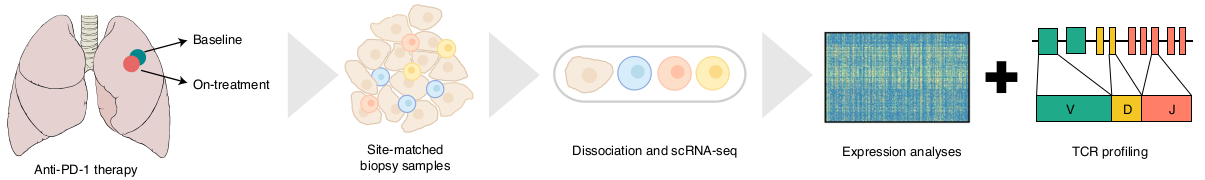
\includegraphics[width=\textwidth]{PD1_NC_01.png}
  \end{figure}
\end{frame}

\begin{frame}
  \frametitle{scRNA | 应用 | 免疫疗法 | 主要结论}
  \begin{block}{主要结论}
      \begin{itemize}
        \item T细胞前体(Texp)的扩张是改善基于 PD-1 抑制剂治疗效果的重要步骤
        \item Texp的扩张最有可能是自我复制以及外周血 T 细胞分化导致的,而不是终末Tex重新激活
      \end{itemize}
  \end{block}
   \begin{figure}
    \centering
    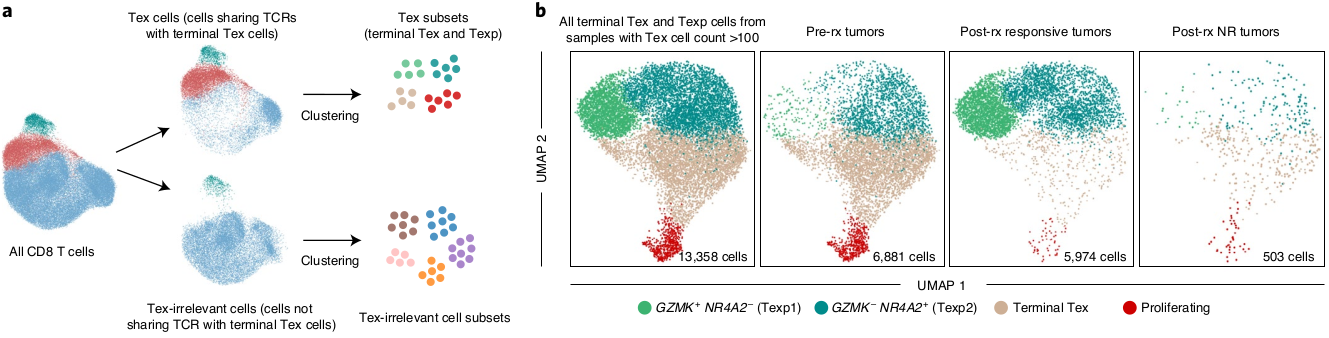
\includegraphics[width=\textwidth]{PD1_NC_02.png}
  \end{figure}
\end{frame}

\begin{frame}
  \frametitle{scRNA | 应用 | 免疫疗法 | 概念突破}
  \begin{block}{“克隆复兴”}
  外周血T细胞补充肿瘤内T细胞的现象。
  \end{block}
   \begin{figure}
    \centering
    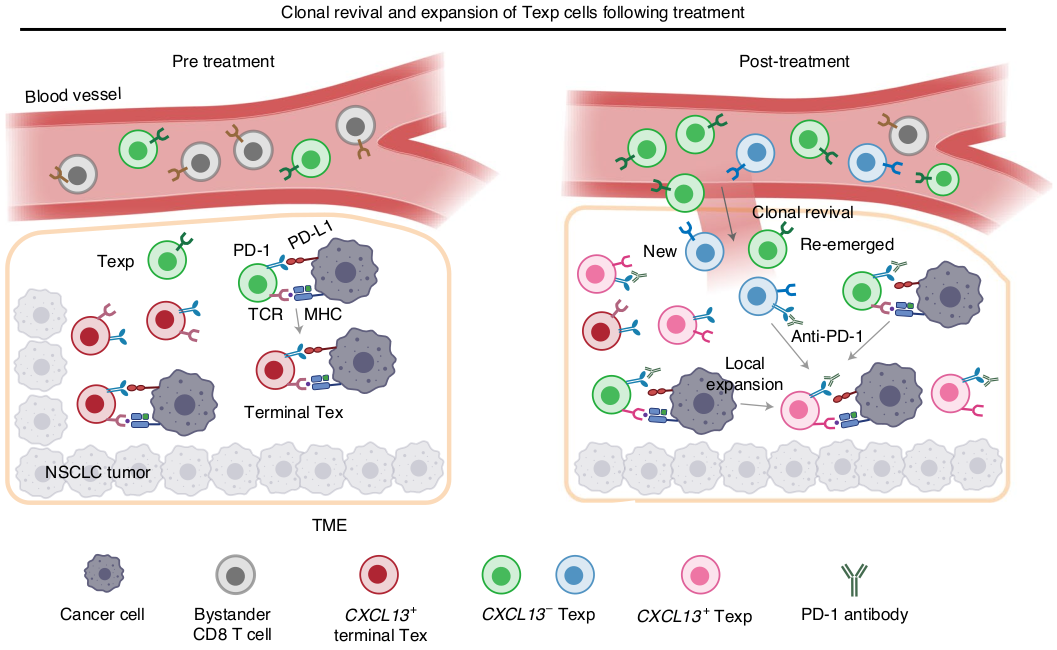
\includegraphics[width=0.9\textwidth]{PD1_NC_03.png}
  \end{figure}
\end{frame}

\subsection{技术简介}
\begin{frame}
  \frametitle{scRNA | 简介}
  \begin{block}{单细胞RNA测序(scRNA-seq,single-cell RNA sequencing)}
  在\alert{单细胞的分辨率水平}上进行 RNA 测序,检测细胞的基因表达水平。\\
  与传统的转录组学测序相比,scRNA-seq技术可以描绘组织块(或细胞悬液)中单个细胞独特的基因表达模式,反映群体的\alert{细胞异质性}。
  \end{block}
     \begin{figure}
    \centering
    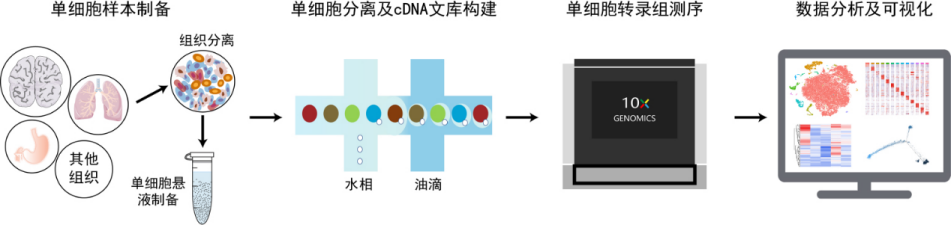
\includegraphics[width=\textwidth]{scRNA_intro_01.png}
  \end{figure}
\end{frame}

\begin{frame}
  \frametitle{scRNA | 简介 |  发展}
    \begin{columns}
  \column{0.48\textwidth}
  \begin{block}{发展简史}
  \begin{itemize}
    \item scRNA-seq技术由\alert{汤富酬}等人在 \alert{2009} 年首次报道。
    \item 随后,Smart-seq、Smart-seq2、Drop-seq等不同平台的技术陆续被开发,该领域迅速繁荣起来。
    \item scRNA-seq已经迅速成为当前生命科学领域\alert{最活跃和前沿}的技术之一。
  \end{itemize}
  \end{block}
  \column{0.58\textwidth}
   \begin{figure}
    \centering
    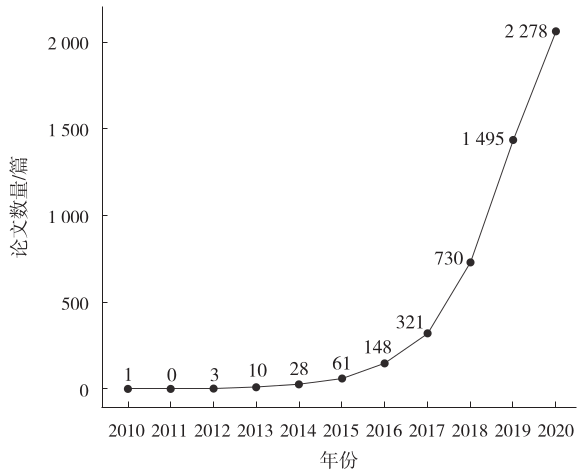
\includegraphics[width=\textwidth]{scRNA_history_01.png}
  \end{figure}
  \end{columns}
\end{frame}

\begin{frame}
  \frametitle{scRNA | 简介 |  发展}
      \begin{columns}
  \column{0.5\textwidth}
  \begin{block}{荣誉}
  \begin{itemize}
    \item 2013年,\textbf{scRNA-seq}被\textit{Nature Methods}杂志列为年度最主要的方法学进展
    \item 2019年,以scRNA-seq为核心代表的\textbf{单细胞多组学方法}再次被\textit{Nature Methods}评选为年度方法
  \end{itemize}
  \end{block}
  \column{0.5\textwidth}
  \begin{block}{应用}
   \begin{figure}
    \centering
    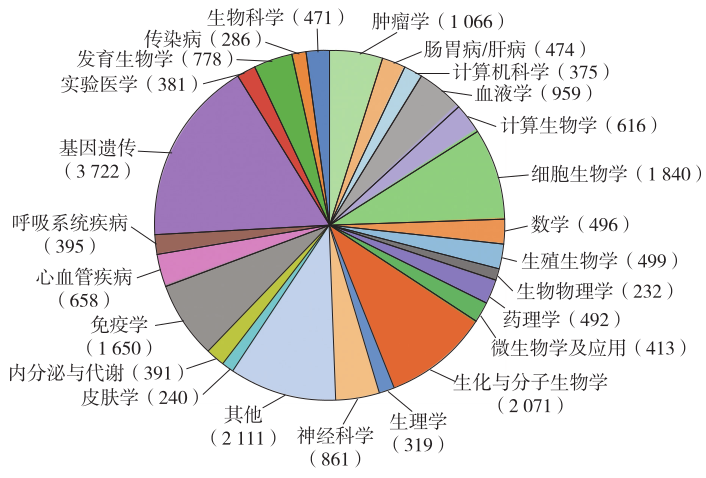
\includegraphics[width=\textwidth]{scRNA_application_01.png}
  \end{figure}
  \end{block}
  \end{columns}
\end{frame}

\begin{frame}
  \frametitle{scRNA | 简介 | 中国人物}
  \begin{columns}
  \column{0.375\textwidth}
     \begin{figure}
    \centering
    \includegraphics[width=\textwidth]{people_Xie.png}
    谢晓亮\\
    (单细胞基因组学的\\开拓者)
  \end{figure}
  \column{0.355\textwidth}
       \begin{figure}
    \centering
    \includegraphics[width=\textwidth]{people_Tang.png}
    汤富酬\\
    (开启了单细胞转录组\\测序时代)
  \end{figure}
  \column{0.32\textwidth}
   \begin{figure}
    \centering
    \includegraphics[width=\textwidth]{people_Zhang.png}
    张泽民\\
    (计算癌症生物学的开拓者与引领者)
  \end{figure}
  \end{columns}
\end{frame}

\begin{frame}
  \frametitle{scRNA | 简介 |  流程}
  \begin{columns}
  \column{0.27\textwidth}
  \begin{block}{scRNA-seq流程}
  \begin{enumerate}
    \item 组织分离
    \item 单细胞捕获
    \item 细胞裂解
    \item 逆转录
    \item 扩增
    \item 文库构建
    \item 测序
    \item 数据分析
  \end{enumerate}
  \end{block}
  \column{0.73\textwidth}
   \begin{figure}
    \centering
    \includegraphics[width=\textwidth]{scRNA_workflow_01.png}
  \end{figure}
  \end{columns}
\end{frame}

\begin{frame}
  \frametitle{scRNA | 简介 |  单细胞捕获技术}
  \begin{columns}
  \column{0.33\textwidth}
  \begin{block}{主流单细胞捕获技术}
  \alert{微流控平台}:
  \begin{itemize}
    \item Drop-seq
    \item InDrop
    \item \alert{Chromium}
    \item ……
  \end{itemize}
  \end{block}
  \column{0.65\textwidth}
      \begin{figure}
    \centering
    \includegraphics[width=\textwidth]{scRNA_compare_01.png}
  \end{figure}
  \end{columns}
  \vspace{-0.3em}
     \begin{figure}
    \centering
    \includegraphics[width=0.75\textwidth]{scRNA_history_02.png}
  \end{figure}
\end{frame}

\subsection{实验原理}
\begin{frame}
  \frametitle{scRNA | 实验 | 微流控平台}
  \begin{block}{微流控平台}
  在油包水的环境下,单细胞与包含特异寡核苷酸标签(barcode)的凝胶珠结合,给每个细胞带上不同的特异性序列,之后将液滴混合、裂解细胞并进行逆转录等后续步骤。
  \end{block}
  \vspace{-0.3em}
       \begin{figure}
    \centering
    \includegraphics[width=0.82\textwidth]{scRNA_tech_01.png}
  \end{figure}
\end{frame}

\begin{frame}
  \frametitle{scRNA | 实验 | Chromium}
    \begin{block}{10x Genomics的Chromium系统}
    利用8通道的微流体“双十字”交叉系统,将含barcode的凝胶珠(Gel Beads)、细胞和酶的混合物、油三者混合,形成GEMs(油包水的微体系),GEMs形成后,细胞裂解,凝胶珠自动溶解释放大量barcode序列。随后mRNA逆转录产生带有10x barcode和UMI信息的cDNA,构建标准测序文库。
  \end{block}
  \vspace{-0.3em}
       \begin{figure}
    \centering
    \includegraphics[width=0.8\textwidth]{scRNA_tech_02.png}
  \end{figure}
\end{frame}

\subsection{分析流程}
\begin{frame}
  \frametitle{scRNA | 分析 | 概览}
  \begin{columns}
  \column{0.55\textwidth}
   \begin{figure}
    \centering
    \includegraphics[width=\textwidth]{scRNA_analysis_workflow_01.png}\\ \vspace{0.5em}
     \includegraphics[width=\textwidth]{scRNA_route.png}
  \end{figure}
  \column{0.45\textwidth}
         \begin{figure}
    \centering
    \includegraphics[width=\textwidth]{scRNA_analysis_workflow_02.png}
  \end{figure}
  \end{columns}
\end{frame}

\begin{frame}
  \frametitle{scRNA | 分析 | 概览}
  \begin{figure}
    \centering
    \includegraphics[width=\textwidth]{scRNA_analysis_workflow_04.png}
  \end{figure}
  \begin{block}{对应关系}
  \begin{itemize}
  \item 微信聊天记录 $\Longrightarrow$ 原始测序数据
  \item 学生 $\Longrightarrow$ 细胞;关键词 $\Longrightarrow$ 基因
  \end{itemize}
  \end{block}
\end{frame}

\begin{frame}
  \frametitle{scRNA | 分析 | 预处理}
  测序后,得到每个单细胞的转录组表达谱,其中由 \alert{barcode标记细胞}、\alert{UMI标记基因}并记录表达量。\\ \vspace{0.5em}
  在对barcode进行分解(demultiplexing)和修剪单次测序所得到的碱基序列reads后,每个barcode分配给特定细胞中特定基因的reads(或使用UMI的分子),再将reads比对到参考基因组,得到单细胞转录组测序的基因的表达矩阵。\\ \vspace{0.5em}
  每个10x样本经 \alert{Cell Ranger} 处理后,将得到 \alert{barcodes.tsv、genes.tsv、matrix.mtx} 3个标准的输出文件。下游处理的时候,必须保证这3个文件同时存在,且在同一个文件夹下。
\end{frame}

\begin{frame}
  \frametitle{scRNA | 分析 | 预处理}
  \begin{block}{Cell Ranger}
 10x genomics公司为单细胞RNA测序分析量身打造的数据分析软件,可以直接输入Illumina原始数据(raw base call,BCL)输出表达定量矩阵、降维(PCA)、聚类(Graph-based \& K-Means)以及可视化(t-SNE)结果,结合配套的Loupe Cell Browser给予研究者更多探索单细胞数据的机会。
 \begin{itemize}
 \item 主要的流程:拆分原始数据mkfastq、细胞表达定量count、定量组合aggr、调参reanalyze
 \item 其他小工具:mkref、mkgtf、upload、sitecheck、mat2csv、vdj、mkvdjref、testrun等
 \end{itemize}
  \end{block}
\end{frame}

\begin{frame}
  \frametitle{scRNA | 分析 | 预处理}
   \begin{figure}
    \centering
    \includegraphics[width=0.95\textwidth]{scRNA_cellranger_01.png}\\ \vspace{0.3em}
    \includegraphics[width=0.37\textwidth]{scRNA_cellranger_02.png}
    \includegraphics[width=0.3\textwidth]{scRNA_cellranger_03.png}
    \includegraphics[width=0.3\textwidth]{scRNA_cellranger_04.png}
  \end{figure}
\end{frame}

\begin{frame}
  \frametitle{scRNA | 分析 | 基本 | 概览}
  \begin{alertblock}{基本分析的主要步骤}
  	\begin{enumerate}
  	\item 质量控制(Quality control):过滤细胞、去除双细胞
  	\item 数据标准化(Normalization):矫正数据、去除批次效应
  	\item 降维(Dimensionality reduction):降低维度、捕获主要信息
  	\item 聚类(Clustering):分群细胞、识别相似群体
  \end{enumerate}
  \end{alertblock}
  \begin{figure}
  	\includegraphics[width=0.95\textwidth]{scRNA_basic_pipeline_01.png}
  \end{figure}
\end{frame}

\begin{frame}
  \frametitle{scRNA | 分析 | 基本 | 质控}
  \begin{block}{质控}
  	数据识别和去除低质量细胞是scRNA-seq质量控制(Quality control, QC)的关键步骤。
  	\end{block}
  \begin{block}{质控建议}
  	在实际操作中,考虑到严格筛选可能删除具有实际意义的细胞,通常会采用较为\alert{松弛的标准进行初筛},在后续分析的过程中再进行二次筛选或人工识别。
  \end{block}
\end{frame}

\begin{frame}
  \frametitle{scRNA | 分析 | 基本 | 质控}
  \begin{columns}
  	\column{0.63\textwidth}
  \begin{block}{质控策略}
  	由于技术和环境等原因,细胞标签(Barcodes)可能会标记doublets、死细胞或外膜破损的细胞。针对这些问题,目前有以下几种解决策略:
  	\begin{itemize}
  	\item 根据每个细胞中转录本的总量或库的大小进行合格细胞的筛选
  	\item 依据线粒体基因读长(Reads)所占的百分比来筛选合格细胞
  	\item 采用Spikein占基因总表达量的比例来判断细胞是否符合标准
  	\item 根据每个基因在所有细胞中表达量的总和来筛选基因
  \end{itemize}
  \end{block}
\column{0.4\textwidth}
  \begin{figure}
	\includegraphics[width=1.1\textwidth]{scRNA_qc_01.png}
\end{figure}
\end{columns}
\end{frame}

\begin{frame}
  \frametitle{scRNA | 分析 | 基本 | 标准化}
  \begin{block}{数据标准化}
  	单细胞RNA测序中,由于细胞之间的异质性及技术因素,各单细胞文库大小和测序深度会有不同,需要通过统计学方法消除这种差异,即数据标准化(Normalization)。
  \end{block}
  \begin{figure}
	\includegraphics[width=\textwidth]{scRNA_normalization_01.png}
\end{figure}
\end{frame}

\begin{frame}
  \frametitle{scRNA | 分析 | 基本 | 标准化}
  \begin{block}{CPM标准化}
  	以 CPM(Counts per million)标准化为例,该方法主要基于如下假设:所有细胞中包含等量的mRNA分子,故所有的Count深度差异全部来自于抽样。CPM标准化后的Count矩阵需要进行对数转换,便于后续的差异表达分析。需要注意的是,对数转换过程中通常会添加一个极小值(如1),以避免对数底数为0。
  \end{block}
 \begin{block}{SCT标准化}
 	SCTransform函数可以代替三个函数(NormalizeData, ScaleData, FindVariableFeatures)的运行。且其对测序深度的校正效果要好于log标准化(10万以内的细胞都建议使用SCT标准化)。SCTransform对测序深度的校正效果很好,也可用于矫正线粒体等因素的影响,但不能用于批次矫正。
\end{block}
\end{frame}

\begin{frame}
  \frametitle{scRNA | 分析 | 基本 | 降维}
  \begin{block}{原因}
  	高维性是scRNA-seq数据的显著特点。
  \end{block}
 \begin{block}{降维}
 	降维(Dimensionality reduction)指将包含冗余信息的高维度的单细胞,在保留有用信息的情况下,降至三维或二维可视化,从而减少大部分的计算量。
\end{block}
 \begin{alertblock}{类型}
 	\begin{itemize}
 		\item 线性降维:PCA(Principal component analysis, 主成分分析)
 		\item 非线性降维
 		\begin{itemize}
 			\item t-SNE(t-distributed stochastic neighbor embedding)
 			\item UMAP(Uniform manifold approximation and projection)
 		\end{itemize}
 	\end{itemize}
\end{alertblock}
\end{frame}

\begin{frame}
  \frametitle{scRNA | 分析 | 基本 | 降维}
  {\footnotesize
  \begin{description}
    \item[PCA] 借助正交变换使线性维数减少,产生一组不相关的分量,通过最大化投影数据的方差,将高维数据投影到低维线性空间上。
  	\item[t-SNE] 通过捕获局部结构,将原始高维空间中不相似单元以大距离建模,而相似单元则以小距离建模,在不丢失数据点间相对距离的基础上,将高维数据嵌入到二维或三维空间中进行可视化。
  	\item[UMAP] 沿着分化轨迹排列簇并保留瞬时细胞的分化连续体,通过在二维或三维图上覆盖标记基因的表达或与生物过程有关的一组基因的活性,捕获scRNA-seq数据中局部和全局结构。
  \end{description}
}
    \begin{figure}
  	\includegraphics[width=\textwidth]{scRNA_dims_01.png}
  \end{figure}
\end{frame}

\begin{frame}
  \frametitle{scRNA | 分析 | 基本 | 聚类}
  \begin{block}{依据}
     相似的细胞具有相似的基因表达谱,因此根据每个细胞中的基因表达情况,可将相似类型的细胞聚集到一起,形成一个细胞簇。
  \end{block}
  \begin{block}{聚类}
	聚类(Clustering)主要是依据细胞-细胞距离矩阵将细胞归属到数目不等的类群中,使高度相似的细胞最大限度地聚为一个类群。
  \end{block}
  \begin{block}{目标}
	聚类的目标是探究或鉴定组织样本中细胞类型或亚型,揭示组织的复杂结构和潜在功能。
\end{block}
\end{frame}

\begin{frame}
  \frametitle{scRNA | 分析 | 基本 | 聚类}
  \begin{columns}
  	\column{0.45\textwidth}
  	    \begin{block}{注意事项}
  		研究者事先并不知原始的所有细胞应该归属于几类以及这些细胞是否具有聚类的意义,因此聚类前用户需要初步判断数据集的聚类趋势。
  	\end{block}
      \begin{figure}
  	\includegraphics[width=\textwidth]{scRNA_clustering_01.png}
  \end{figure}
  \column{0.55\textwidth}
        \begin{figure}
  	\includegraphics[width=\textwidth]{scRNA_clustering_02.png}
  \end{figure}
  \end{columns}
\end{frame}

\begin{frame}
  \frametitle{scRNA | 分析 | 基本 | 工具}
  \begin{block}{\alert{Seurat}}
  	\alert{R} 软件包,用于QC、分析和探索单细胞RNA-seq数据。
  	{\small
  	\begin{itemize}
  		\item 基本分析:质控、细胞筛选、细胞类型鉴定、特征基因选择、差异表达分析、数据可视化,等
  		\item 高级功能:时序单细胞数据分析、多组学单细胞数据整合分析,等
  	\end{itemize}
}
  \end{block}
        \begin{figure}
	\includegraphics[width=0.85\textwidth]{scRNA_seurat.png}
\end{figure}
\end{frame}

\begin{frame}
	\frametitle{scRNA | 分析 | 基本 | 工具}
	\begin{columns}
\column{0.8\textwidth}
	\begin{block}{\alert{Scanpy}}
		基于 \alert{Python} 分析单细胞数据的软件包,包括预处理、可视化、聚类、拟时序分析和差异表达分析等。
	\end{block}
	\column{0.2\textwidth}
     \begin{figure}
		\includegraphics[width=\textwidth]{scRNA_scanpy_logo.png}
	\end{figure}
\end{columns}
	\begin{figure}
		\includegraphics[width=\textwidth]{scRNA_scanpy.png}
	\end{figure}
\end{frame}

\begin{frame}
  \frametitle{scRNA | 分析 | 基本 | 工具}
  	\begin{figure}
   	\includegraphics[width=0.9\textwidth]{scRNA_tools_01.png}
  \end{figure}
\end{frame}


\subsection{分析角度}

\begin{frame}
	\frametitle{scRNA | 分析 | 角度 | 类型注释}
	\begin{columns}
		\column{0.5\textwidth}
	\begin{block}{细胞类型注释}
		在scRNA-seq数据分析中,通过对单个细胞类群的marker基因进行鉴定,可赋予每个类一个有生物学意义的标签,该过程即细胞类型注释。
	\end{block}
\column{0.5\textwidth}
  	\begin{figure}
	\includegraphics[width=\textwidth]{scRNA_celltype_01.png}
\end{figure}
\end{columns}
\pause
    \begin{block}{注释原理}
    	\begin{itemize}
    		\item 鉴定和注释细胞类群主要依赖于外部参考数据库,如Human Cell Atlas、CellMarker、CancerSEA、PanglaoDB等 。
    		\item 在无相关参考库的情况下,可通过现有细胞的标志基因(Marker)和文献报道的特定类型细胞的标志基因进行匹配来鉴定未知细胞的类型。
    	\end{itemize}
    \end{block}
\end{frame}

\begin{frame}
	\frametitle{scRNA | 分析 | 角度 | 类型注释}
	\begin{block}{注释策略:自动注释 vs. 人工注释}
		\begin{itemize}
			\item 人工注释的方法在准确性上要优于自动注释
			\item 自动注释在注释效率和灵敏度上要优于手动注释
			\item 对于较大的数据集来说,现阶段最好的办法是同时进行软件或数据库自动注释及人工注释
			\item 对于细胞类型复杂度较低的数据集而言,人工注释更为经济有效
		\end{itemize}
	\end{block}
\end{frame}

\begin{frame}
	\frametitle{scRNA | 分析 | 角度 | 类型注释}
	\begin{columns}
		\column{0.8\textwidth}
			\begin{block}{SingleR}
			SingleR是一个用于对scRNA-seq数据进行细胞类型自动注释的R包。
		\end{block}
		\column{0.2\textwidth}
		     \begin{figure}
			\includegraphics[width=0.8\textwidth]{scRNA_singler_logo.png}
		\end{figure}
	\end{columns}
    \begin{block}{注释原理}
    	\begin{itemize}
    		\item SingleR通过给定的具有已知类型标签的细胞样本作为参考数据集,对测试数据集中与参考集相似的细胞进行标记注释。
    		\item SingleR自带7个参考数据集,其中5个是人类数据,2个是小鼠的数据。
    	\end{itemize}
    \end{block}
\end{frame}

\begin{frame}
	\frametitle{scRNA | 分析 | 角度 | 类型注释}
	\begin{block}{参考数据集}
		\begin{itemize}
			\item 人类:BlueprintEncodeData;DatabaseImmuneCellExpressionData;HumanPrimaryCellAtlasData;MonacoImmuneData;NovershternHematopoieticData
			\item 小鼠:ImmGenData;MouseRNAseqData
		\end{itemize}
    \end{block}
	\begin{block}{注释过程}
		\begin{enumerate}
			\item 计算每个细胞的表达谱与参考样品的表达谱之间的Spearman相关性。
			\item 将每个标签的分数定义为相关分布的固定分位数。
			\item 对所有的标签重复此操作,然后将得分最高的标签作为此细胞的注释。
		\end{enumerate}
    \end{block}
\end{frame}

\begin{frame}
	\frametitle{scRNA | 分析 | 角度 | 结构推断}
		\begin{columns}
		\column{0.78\textwidth}
		\begin{block}{InferCNV}
		用于肿瘤单细胞RNA-seq数据中鉴定大规模染色体拷贝数变异(copy number alterations, CNA)。
		\end{block}
		\column{0.27\textwidth}
		\begin{figure}
			\includegraphics[width=\textwidth]{scRNA_infercnv_logo.png}
		\end{figure}
	\end{columns}
		\begin{columns}
	\column{0.6\textwidth}
	    \begin{block}{主要应用}
判断肿瘤细胞;分析肿瘤异质性;探索克隆进化
	\end{block}
    \begin{block}{基本原理}
    	在整个基因组范围内,将每个肿瘤细胞基因表达与平均表达或 “正常” 参考细胞基因表达对比,确定其表达强度,分析肿瘤基因组上各个位置的基因表达量强度变化。
    \end{block}
\column{0.4\textwidth}
\begin{figure}
	\includegraphics[width=\textwidth]{scRNA_infercnv.png}
\end{figure}
	\end{columns}
\end{frame}

\begin{frame}
	\frametitle{scRNA | 分析 | 角度 | 轨迹推断}
	\begin{block}{拟时序分析法}
		根据单个细胞的基因表达模式推断出细胞发育或分化的动态路径。\textbf{注意分析结果不一定代表实际的细胞分化过程。}
    \end{block}
\pause
    \begin{columns}
    	\column{0.68\textwidth}
    	\begin{block}{基本原理}
    		通常scRNA-seq技术只能描绘在某一时刻细胞中的基因转录表达状态,只能得到一张细胞的“快照”。而“伪时间(pseudotime)”可以近似作为衡量细胞分化发育的相对次序,该次序通过对细胞间表达谱的相似性计算和推测得到。随后,这些细胞将会按照这种相对次序被分配到一个一维空间中,代表着细胞发育分化进程中的一种独特状态。
    	\end{block}
    	\column{0.4\textwidth}
    	\begin{figure}
    		\includegraphics[width=\textwidth]{scRNA_pseudotime.png}
    	\end{figure}
    \end{columns}
\end{frame}

\begin{frame}
	\frametitle{scRNA | 分析 | 角度 | 轨迹推断}
	\begin{block}{Monocle}
		首个用于不同分化阶段对细胞排序且兼具鲁棒性和高效性的软件。
	\end{block}
     \begin{columns}
    	\column{0.76\textwidth}
    	\begin{block}{基本原理}
    		在细胞分化发育的过程中都会执行一套特定的基因表达程序,而在整体的生物学过程中,各个细胞执行这套程序往往是不同步的,Monocle正是利用了这一特点,将测序得到的细胞放置在计算得到的一条轨迹上,从而刻画出生物学过程(如发育分化等)中细胞的伪时序发展路径,并进一步提供聚类和差异表达分析等手段帮助我们更好得理解生物过程发展和调控的机制。
    	\end{block}
    	\column{0.26\textwidth}
    	\begin{figure}
    		\includegraphics[width=\textwidth]{scRNA_monocle_01.png}
    		\includegraphics[width=\textwidth]{scRNA_monocle_02.png}
    	\end{figure}
    \end{columns}
\end{frame}

\begin{frame}
	\frametitle{scRNA | 分析 | 角度 | 轨迹推断}
	\begin{block}{RNA速率(RNA velocity)}
		\begin{itemize}
			\item 基因表达状态的时间导数
			\item 通过区分scRNA-seq中未剪接和剪接的mRNA来直接估计
			\item 可以在数小时的时间尺度上预测单个细胞的未来状态
			\item velocyto是RNA 速率分析的常用工具
		\end{itemize}
	\end{block}
\pause
         \begin{columns}
    	\column{0.5\textwidth}
    	\begin{block}{基本原理}
           通过计算细胞内mRNA剪切前后的比例来估算RNA丰度随时间的变化,可以用于细胞分化、谱系发育、肿瘤微环境中细胞成分的动态轨迹变化等研究。
    	\end{block}
    	\column{0.5\textwidth}
    	\begin{figure}
    		\includegraphics[width=\textwidth]{scRNA_velocity.png}
    	\end{figure}
    \end{columns}
\end{frame}

\begin{frame}
	\frametitle{scRNA | 分析 | 角度 | 细胞通讯}
	\begin{block}{细胞通讯分析}
		根据不同细胞膜表面和游离蛋白之间的配体-受体关系,鉴定不同细胞之间可能的相互作用。
	\end{block}
   \begin{columns}
   	\column{0.5\textwidth}
   	\begin{block}{细胞-细胞互作(Cell-cell interaction, CCI)}
   		作为生命活动的基本单位,细胞与细胞之间能通过表面受体-配体蛋白识别结合,并以旁分泌和自分泌等方式传递信号,调控受体细胞的分化、凋亡以及有丝分裂等过程,因此CCI网络在整个生命活动中发挥着重要作用。
   	\end{block}
   	\column{0.5\textwidth}
   	\begin{figure}
   		\includegraphics[width=\textwidth]{scRNA_CCI_01.png}
   	\end{figure}
   \end{columns}
\end{frame}

\begin{frame}
	\frametitle{scRNA | 分析 | 角度 | 细胞通讯}
	\begin{block}{scRNA-seq细胞通讯分析}
		\begin{description}
			\item[主要目标] 比较不同样品组的细胞在各细胞类型之间的配体与受体基因表达差异。
			\item[基本思路] 从单细胞基因表达矩阵出发,结合已有的配体-受体信息,量化配体-受体相互作用的强度,进而推测细胞间的互作关系。
			\item[常用工具] CellPhoneDB、CellTalker、iTALK 和 CellChat等。
		\end{description}
    \end{block}
		\begin{columns}
	\column{0.77\textwidth}
	\begin{block}{CellChat}
         开源R包,主要用于细胞间通讯的分析和可视化。它使用配体受体对应的基因表达对来量化细胞间的相互作用。
	\end{block}
	\column{0.27\textwidth}
	\begin{figure}
		\includegraphics[width=\textwidth]{scRNA_cellchat_logo.png}
	\end{figure}
\end{columns}
\end{frame}

\begin{frame}
	\frametitle{scRNA | 分析 | 角度 | 细胞通讯}
		\begin{description}
			\item[CellphoneDB] 储存受体、配体以及两种相互作用的数据库,考虑了结构组成,能够描述异构复合物。(配体-受体 + 多聚体)
			\item[iTALK] 通过平均表达量方式,筛选高表达的配体和受体,根据结果作圈图。(配体-受体)
			\item[CellChat] 将基因表达数据作为输入,结合配体受体及其辅助因子的相互作用来模拟细胞间通讯。(配体-受体 + 多聚体 + 辅因子)
			\item[NicheNet] 通过将相互作用细胞的表达数据与信号和基因调控网络的先验知识相结合来预测相互作用细胞之间的配体-靶标联系的方法。(配体-受体 + 信号通路)
			\item[Celltalker] 通过寻找细胞群内和细胞群之间已知的配体和受体对的表达来评估细胞间的交流。(配体-受体)
		\end{description}
\end{frame}

\begin{frame}
	\frametitle{scRNA | 分析 | 角度 | 细胞通讯}
	\begin{figure}
		\includegraphics[width=\textwidth]{scRNA_cellchat_01.png}\\
		\vspace{0.5em}
		\includegraphics[width=\textwidth]{scRNA_cellchat_02.png}
	\end{figure}
\end{frame}

\begin{frame}
	\frametitle{scRNA | 分析 | 角度 | 调控网络}
	\begin{columns}
	\column{0.6\textwidth}
	\begin{block}{转录调控网络}
		基因转录调控网络描述转录因子及其调控的基因之间的关系。\\
		阐明转录调控网络的结构和功能是很多研究的核心目标,该项研究面临的挑战主要是重建调控网络,因为基因或转录本代表的节点或边界之间都是相互作用。
	\end{block}
\column{0.4\textwidth}
	\begin{figure}
	\includegraphics[width=\textwidth]{scRNA_network_01.png}
\end{figure}
\end{columns}
		\begin{columns}
	\column{0.7\textwidth}
	\begin{block}{SCENIC}
  识别转录因子与潜在靶基因之间的共表达模块(\textbf{regulon})。
	\end{block}
	\column{0.3\textwidth}
	\begin{figure}
		\includegraphics[width=\textwidth]{scRNA_scenic_logo.png}
	\end{figure}
\end{columns}
\end{frame}

\begin{frame}
	\frametitle{scRNA | 分析 | 角度 | 调控网络}
	\begin{block}{SCENIC}
		SCENIC可以得到细胞类型中regulon的活性强度,找出regulon与每种细胞类型之间特定的对应关系。同时可获得不同regulon之间的关联性,具有较高关联性的regulon可能共同调控下游基因,并共同负责细胞功能。
	\end{block}
\vspace{-0.3em}
\pause
    \begin{columns}
    	\column{0.82\textwidth}
    	\begin{enumerate}
    		\item GENIE3运用随机森林推断潜在的转录因子靶标。
    		\item RcisTarget分析每个regulon的基因,以鉴定富集的motif。\textbf{每个转录因子及其潜在的直接靶标被称为一个regulon。}
    		\item AUCell使用AUC来计算输入基因集的关键子集是否在每个细胞的表达基因中富集,为细胞间的regulon打分赋值。
    		\end{enumerate}
    	\column{0.22\textwidth}
\begin{figure}
\hspace{-1.8em}\includegraphics[width=\textwidth]{scRNA_scenic_01.png}
\end{figure}
    \end{columns}
\end{frame}

\begin{frame}
	\frametitle{scRNA | 分析 | 资料合辑}
	\begin{block}{scRNA-seq分析资料与工具合辑}
		\begin{itemize}
			\item \href{https://github.com/mdozmorov/scRNA-seq_notes}{scRNA-seq data analysis tools and papers}: Single-cell RNA-seq related tools and genomics data analysis resources.
			\item  \href{https://github.com/seandavi/awesome-single-cell}{awesome-single-cell}: List of software packages (and the people developing these methods) for single-cell data analysis, including RNA-seq, ATAC-seq, etc.
			\item  \href{https://github.com/scRNA-tools/scRNA-tools}{scRNA-tools}: A database of software tools for the analysis of single-cell RNA-seq data.
		\end{itemize}
		\end{block}
	\begin{figure}
		\includegraphics[width=0.38\textwidth]{github_logo_04.png}\\
		\vspace{0.5em}
		\includegraphics[width=0.5\textwidth]{scRNA_tools_logo.png}
	\end{figure}
\end{frame}


\section{空间转录组学}
\subsection{技术简介}
\begin{frame}
	\frametitle{ST | 导言 | vs. scRNA}
	\begin{block}{基因表达:动态 + 时空异质性}
		\begin{description}
			\item[传统的转录组测序] 将RNA的表达量平均化,忽略了细胞群体内不同细胞之间基因表达的异质性。
			\item[单细胞RNA测序] 能够独立地提供每个细胞的RNA表达谱,区分出细胞之间的基因表达差异,并鉴定出异质细胞群中的稀有
			细胞;需要将细胞从组织中解离,从而导致细胞空间位置信息
			的丢失。
			\item[空间转录组]  记录所检测RNA分子的空间位置信息。
		\end{description}
	\end{block}
	\begin{figure}
		\includegraphics[width=0.53\textwidth]{ST_vs_scRNA_04.png}
		\includegraphics[width=0.45\textwidth]{ST_vs_scRNA_07.png}
	\end{figure}
\end{frame}

\begin{frame}
    \frametitle{ST | 导言 | 简介}
    \begin{block}{\alert{空间转录组(Spatial transcriptomics,ST)}}
    	结合成像、生物标记、测序及生物信息学等工具对组织切片的基因表达进行空间定位的一项技术,可揭示各细胞类型在组织中的空间分布、各细胞群体间的相互作用以及绘制不同组织区域的基因表达图谱,对于理解疾病和癌症的发生机制具有深远的应用价值。
    \end{block}
	\begin{figure}
	\includegraphics[width=0.9\textwidth]{ST_intro_02.png}
\end{figure}
\end{frame}

\begin{frame}
	\frametitle{ST | 导言 | 历史}
	\begin{block}{技术发展}
		\begin{itemize}
			\item 一系列能够进行高通量原位RNA检测分析的技术都被归为空间转录组学技术的范畴
			\item 空间转录组的发展可以追溯到1969年的原位杂交技术(\textit{in situ} hybridization, ISH)的应用
			\item 2020年,“空间转录组技术”被\textit{Nature Methods}评为年度技术方法
			\item 2022年,空间多组学被\textit{Nature}评为值得关注的七大技术之一
		\end{itemize}
	\end{block}
\vspace{-0.5em}
	\begin{figure}
	\includegraphics[width=0.95\textwidth]{ST_history_03.png}
\end{figure}
\end{frame}

\begin{frame}
	\frametitle{ST | 导言 | 技术}
	\begin{block}{技术概述}
		根据空间转录组获取空间信息的原理不同,分为四类:
		\begin{description}
			\item[显微切割技术] 在显微镜下通过手工操作或仪器采样的方法从组织切片或细胞图片上将所研究的目标细胞从中分离出来。
			\item[原位杂交技术] 使用\textcolor{gray}{同位素标记或}荧光标记的探针与预定的靶RNA/DNA杂交,确定组织或细胞中的RNA/DNA丰度,逐渐发展至单分子分辨水平。
			\item[原位测序技术] 利用单碱基特异性荧光杂交和DNA连接反应对组织中已知或未知转录本的序列进行原位测定。
			\item[\alert{原位捕获技术}] 利用具有空间位置信息的DNA标签引物捕获并标记转录本的空间位置。
		\end{description}
	\end{block}
\end{frame}

\begin{frame}
	\frametitle{ST | 导言 | 技术}
		\begin{figure}
		\includegraphics[width=0.8\textwidth]{ST_tech_01.png}
	\end{figure}
\end{frame}

\begin{frame}
	\frametitle{ST | 导言 | 应用}
			\begin{figure}
		\includegraphics[width=0.8\textwidth]{ST_application_01.png}
		\includegraphics[width=0.8\textwidth]{ST_application_05.png}
	\end{figure}
\end{frame}

\begin{frame}
	\frametitle{ST | 导言 | 升华}
	\begin{figure}
		\includegraphics[width=0.85\textwidth]{ST_vs_scRNA_05.png}\\
		\vspace{0.3em}
		\includegraphics[width=0.85\textwidth]{ST_vs_scRNA_08.png}
	\end{figure}
\end{frame}

\subsection{应用案例}
\begin{frame}
	\frametitle{ST | 应用 | 器官发生}
	\begin{block}{器官发生}
		器官发生(Organogenesis)亦称器官形成,一般指脊椎动物个体发育中,由器官原基进而演变为器官的过程。各种器官形成的时间有早有晚,通过器官发生阶段,各种器官经过形态发生和组织分化, 逐渐获得了特定的形态并执行一定的生理功能。
		\end{block}
		\begin{figure}
		\includegraphics[width=0.85\textwidth]{ST_development_01.png}
	\end{figure}
\end{frame}

\begin{frame}
	\frametitle{ST | 应用 | 心脏发育}
		\begin{block}{心脏发育}
			心脏发育( Heart development),也称为心脏发生(Cadiogenesis ),指的是人类心脏的产前发育。心脏发育从两个心内膜管的形成开始,两个心内膜管合并形成被称为原始心血管的管状心脏,管状心脏通过四个腔室和成对的动脉干发育形成成年心脏。
	\end{block}
	\begin{figure}
		\includegraphics[width=0.85\textwidth]{ST_development_heart_01.png}
	\end{figure}
\end{frame}

\begin{frame}
	\frametitle{ST | 应用 | 心脏发育}
	\begin{block}{研究背景}
		心脏是人类胚胎发育过程中第一个完全功能化的实质器官。其复杂的发育过程,如从中胚层中分化出心管、心管弯曲形成四个腔体、流出道分化成主动脉与肺动脉等,尽管在大体层面已经得到较好的刻画,但在细节上的动态变化,尤其是全器官尺度上的,仍未得到完全解析。
		\end{block}
	\vspace{-0.3em}
		\begin{figure}
		\includegraphics[width=\textwidth]{ST_heart_01.png}\\
		\vspace{-0.6em}
		\includegraphics[width=\textwidth]{ST_heart_02.png}
	\end{figure}
\end{frame}

\begin{frame}
	\frametitle{ST | 应用 | 心脏发育}
			\begin{figure}
		\includegraphics[width=0.9\textwidth]{ST_heart_07.png}
	\end{figure}
\end{frame}

\begin{frame}
	\frametitle{ST | 应用 | 心脏发育}
	\begin{figure}
		\includegraphics[width=0.34\textwidth]{ST_heart_05.png}
	    \includegraphics[width=0.63\textwidth]{ST_heart_06.png}\\
	    \includegraphics[width=\textwidth]{ST_heart_04.png}
	\end{figure}
\end{frame}

\begin{frame}
	\frametitle{ST | 应用 | 心脏发育}
	\begin{columns}
		\column{0.51\textwidth}
		\begin{block}{研究总结}
			采集妊娠早期3个阶段(孕4.5~5.0周,6.5周和9.0周)的心脏组织样本,采用单细胞测序结合ST和ISS技术绘制了心脏发育过程中基因表达的时空图谱。ST与ISS技术联合确定了发育过程中不同的解剖区域特异的基因表达谱,而单细胞RNA测序则帮助鉴定了细胞的类型,并通过联合分析映射到特定的解剖区域,最终构建了妊娠早期3个阶段心脏发育的三维可视化转录图谱。
			\end{block}
    \column{0.55\textwidth}
	\begin{figure}
		\includegraphics[width=\textwidth]{ST_heart_03.png}
	\end{figure}
	\end{columns}
\end{frame}


\subsection{实验原理}
\begin{frame}
	\frametitle{ST | 实验 | ST}
	\begin{block}{原位捕获技术}
		原位捕获技术的核心是利用具有空间位置信息的DNA标签引物捕获并标记转录本的空间位置。\\
		近几年原位捕获技术发展迅猛,并朝着\alert{提高空间分辨率及空间多组学联合分析}两个方向发展。
		\end{block}
		\begin{block}{空间转录组(Spatial transcriptomics, ST)}
       \begin{itemize}
       	\item 2016年首次提出
       	\item 能够在单个组织切片上提供mRNA分布的可视化和基因表达数据
       	\item 2018年被10x Genomics收购并更名为 \alert{10x Visium}
       \end{itemize}
	\end{block}
\end{frame}

\begin{frame}
	\frametitle{ST | 实验 | Visium}
		\begin{block}{基本原理}
			将含有空间编码、分子编码的mRNA特异捕获引物簇固定于载玻片表面以制备空间编码玻片;接着将组织切片贴于空间编码玻片,并对其进行固定、染色与成像;利用玻片上的引物捕获经透化后的组织释放的mRNA,通过逆转录过程生成含有空间编码的cDNA,经转录组文库制备、高通量测序与分析,将转录组序列映射至原空间位置,实现高覆盖度的组织空间转录组测量分析。
	\end{block}
\vspace{-0.6em}
		\begin{figure}
	\includegraphics[width=\textwidth]{ST_workflow_08.png}
\end{figure}
\end{frame}

\begin{frame}
	\frametitle{ST | 实验 | Visium}
		\begin{figure}
		\includegraphics[width=\textwidth]{ST_workflow_04.png}
	\end{figure}
\vspace{-0.5em}
	\begin{figure}
		\includegraphics[width=\textwidth]{ST_workflow_06.png}
	\end{figure}
\end{frame}

\begin{frame}
	\frametitle{ST | 实验 | Visium}
	\begin{block}{技术要点}
		\begin{itemize}
			\item 一个载玻片可容纳4个切片(捕获区域),制备4个文库
			\item 每个捕获区域大小为6.5mm x 6.5mm
			\item 每个捕获区域有5000个barcode标记的ST位点
			\item 每个ST位点直径55 \textmu m,点与点之间相距100 \textmu m
			\item 每个ST位点覆盖1-10个细胞\alert{(非单细胞水平)}
			\item 每个ST位点有百万个UMI探针,检测数千个基因
		\end{itemize}
		\end{block}
	\vspace{-0.5em}
		\begin{figure}
		\includegraphics[width=0.9\textwidth]{ST_design_01.png}
	\end{figure}
\end{frame}

\subsection{分析策略}
\begin{frame}
	\frametitle{ST | 分析 | 概览}
	\begin{figure}
	\includegraphics[width=\textwidth]{ST_tools.png}
   \end{figure}
\end{frame}

\begin{frame}
	\frametitle{ST | 分析 | 概览}
	\begin{figure}
	\includegraphics[width=\textwidth]{ST_route.png}
    \end{figure}
\end{frame}

\begin{frame}
	\frametitle{ST | 分析 | Space Ranger}
	\begin{block}{Space Ranger}
	利用10x Genomics官方分析流程及软件(Space Ranger \& Loupe Browser),可将细胞分群信息与其空间定位相结合,深入探索不同空间定位下特定细胞亚群的生物学功能。
	\end{block}
    \begin{figure}
    	\includegraphics[width=\textwidth]{ST_spaceranger_02.png}
    \end{figure}
\end{frame}
% spaceranger count从spaceranger mkfastq中获取明场切片图像和FASTQ文件,并执行对齐,组织检测,基准检测和条形码/UMI 计数。该管道使用Visium空间条形码生成特征点矩阵feature-spot matrices,确定聚类并执行基因表达分析。

\begin{frame}
	\frametitle{ST | 分析 | Space Ranger}
	\begin{figure}
		\includegraphics[width=0.56\textwidth]{ST_spaceranger_01.png}
		\includegraphics[width=0.41\textwidth]{ST_spaceranger_03.png}\\
		\vspace{0.5em}
		\includegraphics[width=\textwidth]{ST_spaceranger_05.png}
	\end{figure}
\end{frame}

\begin{frame}
	\frametitle{ST | 分析 | Seurat}
		\begin{block}{Seurat}
			应用Seurat分析空间转录组的流程类似于scRNA-seq分析,但引入了更新的交互和可视化工具,特别强调了空间和分子信息的整合。
			\begin{itemize}
				\item 标准化、降维和聚类
				\item 检测空间高变基因;处理多个切片;交互式可视化
				\item 与单细胞RNA-seq数据整合
			\end{itemize}
	\end{block}
\vspace{-1em}
	\begin{figure}
		\includegraphics[width=0.9\textwidth]{ST_seurat_01.png}
	\end{figure}
\end{frame}

\begin{frame}
	\frametitle{ST | 分析 | Giotto}
		\begin{block}{Giotto}
	Giotto提供了一个全面的空间分析工具箱,包含两个独立但完全集成的模块。 第一个模块(Giotto Analyzer)提供有关分析空间单细胞表达数据的不同步骤的分析说明,第二个模块(Giotto Viewer)在用户本地计算机上提供此类数据的响应式和交互式查看器。
	\end{block}
\vspace{-0.5em}
		\begin{figure}
		\includegraphics[width=0.85\textwidth]{ST_gitto_01.png}
	\end{figure}
\end{frame}

\begin{frame}
	\frametitle{ST | 分析 | 深度学习}
	\begin{figure}
		\includegraphics[width=\textwidth]{ST_deeplearning_01.png}
	\end{figure}
\end{frame}


\section{单细胞多组学}
\subsection{其他单细胞组学}
\begin{frame}
	\frametitle{其他 | 组学}
	\begin{block}{组学(Omics )}	
		通常指生物学中对各类研究对象(一般为生物分子)的集合所进行的系统性研究,例如基因组学、蛋白质组学和代谢物组学等,而这些研究对象的集合被称为组。
	\end{block}
	\begin{figure}
	\includegraphics[width=\textwidth]{omics_08.png}
\end{figure}
\end{frame}

\begin{frame}
	\frametitle{其他 | 组学}
		\begin{figure}
		\includegraphics[width=\textwidth]{omics_03.png}
	\end{figure}
\end{frame}

\begin{frame}
	\frametitle{其他 | 单细胞组学}
	\begin{figure}
		\includegraphics[width=\textwidth]{omics_10.png}
	\end{figure}
\end{frame}

\begin{frame}
	\frametitle{其他 | scATAC-seq}
	\begin{block}{ATAC-seq}
            ATAC-seq是用于检测基因组染色质可及性的分子生物学手段。ATAC-seq分析可以用于研究许多染色质可及性特征。最常见的用途是核小体定位,也可用于定位转录因子结合位点。
	\end{block}
		\begin{figure}
		\includegraphics[width=\textwidth]{scATAC_01.png}
	\end{figure}
\end{frame}

\begin{frame}
	\frametitle{其他 | scATAC-seq}
	\begin{figure}
		\includegraphics[width=\textwidth]{scATAC_03.png}
	\end{figure}
\end{frame}

\begin{frame}
	\frametitle{其他 | scChIP-seq}
	\begin{block}{ChIP-seq}
		ChIP-seq被用于分析蛋白质与DNA的交互作用。该技术将染色质免疫沉淀(ChIP)与大规模并行DNA测序结合起来以鉴定与DNA相关蛋白的结合部位。可被用于精确绘制任意目的蛋白在全基因组上的结合位点,以确定转录因子和其他染色质相关蛋白质如何影响表型影响机制。
	\end{block}
	\begin{figure}
	\includegraphics[width=\textwidth]{scChIP-seq_01.png}
\end{figure}
\end{frame}

\begin{frame}
	\frametitle{其他 | scHi-C}
	\begin{columns}
		\column{0.52\textwidth}
			\begin{block}{Hi-C}
				Hi-C技术源于染色体构象捕获(3C)技术,利用高通量测序技术,结合生物信息分析方法,研究全基因组范围内整个染色质DNA在空间位置上的关系,获得高分辨率的染色质三维结构信息。最初用于捕获全基因组范围内所有的染色质内和染色质间的空间互作信息,目前已应用于基因表达的空间调控机制研究、构建染色体水平参考基因组、构建单体型图谱等。
		\end{block}
	\column{0.55\textwidth}
				\begin{figure}
		\includegraphics[width=\textwidth]{scHi-C_03.png}
	\end{figure}
	\end{columns}
\end{frame}

\begin{frame}
	\frametitle{其他 | Perturb-seq}
	\begin{block}{Perturb-seq}
		利用CRISPR-Cas9技术将基因变化引入细胞内,然后使用单细胞转录组测序捕获特定基因变化导致的转录组信息变化,能够研究给定细胞类型的全面遗传扰动影响,可以以前所未有的深度跟踪打开或关闭基因的影响。
		\end{block}
				\begin{figure}
		\includegraphics[width=0.56\textwidth]{perturb-seq_01.png}
		\includegraphics[width=0.41\textwidth]{perturb-seq_03.png}
	\end{figure}
\end{frame}

\begin{frame}
	\frametitle{其他 | scMS}
			\begin{figure}
		\includegraphics[width=0.8\textwidth]{scMS.png}
	\end{figure}
\end{frame}

\begin{frame}
	\frametitle{其他 | 单细胞组学 | 应用}
		\begin{figure}
		\includegraphics[width=\textwidth]{sc_application_01.png}
	\end{figure}
\end{frame}

\begin{frame}
	\frametitle{其他 | 单细胞组学 | 应用}
			\begin{figure}
		\includegraphics[width=\textwidth]{sc_application_02.png}
	\end{figure}
\end{frame}

\subsection{单细胞多组学}
\begin{frame}
	\frametitle{多组学 | 简介}
	\begin{columns}
		\column{0.53\textwidth}
		\begin{block}{多组学(Multiple omics)}	
			多组学提供了一个综合视角,这种分析方法将基因组数据与转录组学、表观遗传学、蛋白质组学其他模式的数据相结合,可测量基因表达、基因激活和蛋白质水平。\\ \vspace{0.4em}
			多组学分析研究能够帮助我们更全面地了解分子变化对正常发育、细胞响应和疾病的影响。研究人员可以借助多组学技术更好地将基因型与表型联系起来,不断探索、发现新药物靶点和生物标志物。
		\end{block}
	\column{0.55\textwidth}
		\begin{figure}
		\includegraphics[width=\textwidth]{omics_05.png}
	\end{figure}
	\end{columns}
\end{frame}

\begin{frame}
	\frametitle{多组学 | 简介}
	\begin{figure}
		\includegraphics[width=0.45\textwidth]{omics_02.png}
		\includegraphics[width=0.53\textwidth]{omics_04.png}
	\end{figure}
\end{frame}

\begin{frame}
	\frametitle{多组学 | 简介}
	\begin{figure}
	\includegraphics[width=\textwidth]{omics_06.png}
    \end{figure}
\end{frame}

\begin{frame}
	\frametitle{单细胞多组学 | 简介}
	\begin{columns}
		\column{0.55\textwidth}
	\begin{block}{单细胞多组学}
		单细胞多组学技术通过测量来自同一单个细胞的多种分子,包括 DNA、RNA、染色质和蛋白质分子等,整合来自多个组学水平的信息,可以为同一细胞构建多组学概况。
	\end{block}
		\column{0.55\textwidth}
	\begin{figure}
	\includegraphics[width=\textwidth]{multimodel_02.png}
\end{figure}
\end{columns}
    \begin{block}{优势}
    	\begin{itemize}
    		\item 单细胞多组学技术是单细胞分析技术发展的前沿,也是单组学技术发展的必然趋势。
    		\item 与细胞的单组学相比,多组学更侧重对细胞完整信息的采集以及对时间空间的关注,因此可以更好和更全面地反映细胞特征,可提供更准确的生物学见解。
    	\end{itemize}
    \end{block}
\end{frame}

\begin{frame}
	\frametitle{单细胞多组学 | 策略}
	\begin{figure}
		\includegraphics[width=0.8\textwidth]{multimodel_03.png}
	\end{figure}
\end{frame}

\begin{frame}
	\frametitle{单细胞多组学 | 多模态}
	\begin{figure}
		\includegraphics[width=0.8\textwidth]{multimodel_01.png}
	\end{figure}
\end{frame}

\begin{frame}
	\frametitle{单细胞多组学 | 双组学}
	\begin{block}{单细胞转录组和基因组联合分析}
		\begin{itemize}
			\item 基因组是决定细胞内遗传变异分子机制的源代码,而转录组决定了细胞的特定功能。
			\item 基因组和转录组的联合分析通过探究DNA拷贝数、DNA编码区与非编码区如何决定转录组表达水平,从而建立基因组和转录组的相关性,并阐述选择性表达分子作用机制,如RNA编辑、调控变异和等位基因特异性表达。
			\item 对不同细胞的基因组和转录组进行联合分析,可进一步\alert{区分遗传亚克隆},同时进行谱系示踪。
		\end{itemize}
	\end{block}
\end{frame}

\begin{frame}
	\frametitle{单细胞多组学 | 双组学}
		\begin{block}{单细胞转录组和蛋白质组联合分析}
					\begin{itemize}
				\item 蛋白质作为表型的直接输出者,直接反映细胞当下的生理状态和细胞功能。
				\item 转录组和蛋白质组的联合测量有助于解释转录异质性如何转化为功能表型多样性,深入理解转录/翻译后修饰过程。
				\item 有助于\alert{揭示RNA层面无法区分的表型差异},并探讨特定细胞亚型的基因表达网络和功能调控类型。
			\end{itemize}
	\end{block}
\end{frame}

\begin{frame}
	\frametitle{单细胞多组学 | 双组学}
		\begin{block}{单细胞转录组和表观遗传组联合分析}
			{\small
					\begin{itemize}
				\item 细胞内表观遗传标记变化广泛,如DNA甲基化修饰、组蛋白修饰、转录因子结合、染色质可及性等,其通过调节染色质结构与构象促进/抑制转录组表达。
				\item 对转录组和表观基因组进行联合分析可以解析染色质结构与构象变化对细胞基因表达的可塑性,并构建细胞表观遗传调控网络,揭示基因表达调控机制。二者的同时分析可帮助鉴别细胞发育和疾病发展过程中的特殊标记并实现遗传谱系示踪。
				\item 染色质可及性和转录组的联合检测为\alert{揭示单个细胞的基因调控机制}提供了强有力的工具。
				\item 单细胞DNA甲基化组和转录组的联合分析可鉴别突变产生的遗传谱系,全面揭示细胞间的异质性,同时探讨DNA甲基化修饰对基因表达的调控规律。
			\end{itemize}
		}
	\end{block}
\end{frame}

\begin{frame}
	\frametitle{单细胞多组学 | 双组学}
	\begin{figure}
		\includegraphics[width=\textwidth]{scRNA_scATAC_01.png}\\
        \includegraphics[width=0.98\textwidth]{scRNA_scATAC_02.png}
	\end{figure}
\end{frame}

\begin{frame}
	\frametitle{单细胞多组学 | 双组学}
	\begin{figure}
		\includegraphics[width=\textwidth]{scRNA_scATAC_03.png}
	\end{figure}
\end{frame}

\begin{frame}
	\frametitle{单细胞多组学 | 双组学 | 两种策略}
	\begin{figure}
		\includegraphics[width=\textwidth]{scRNA_scATAC_05.png}
	\end{figure}
\end{frame}

\begin{frame}
		\frametitle{单细胞多组学 | 三组学}
			\begin{block}{scTrio-seq}
				\begin{itemize}
					\item 首次同时分析了单个哺乳动物细胞中基因组、DNA 甲基化和转录组之间的关系,可以获取单个细胞的拷贝数变异、DNA甲基化和转录组信息。
					\item 以10 Mb分辨率准确推导CNV模式,获得了150万个CpG位点的甲基化模式,并检测了单个哺乳动物细胞中平均6179个基因的表达水平。
					\item 分析了来自人类肝细胞癌组织样品的25个单细胞,发现2个细胞亚群的DNA拷贝数、DNA甲基化或RNA表达水平不同;通过比较2个HCC亚群之间的多基因组差异,发现某一亚群具有更多的拷贝数变异,表达了更多的侵袭性细胞标志物,且更有可能逃避免疫监视。
				\end{itemize}
		\end{block}
\end{frame}

\begin{frame}
	\frametitle{单细胞多组学 | 三组学}
		\begin{figure}
		\includegraphics[width=\textwidth]{scTrio-seq.png}
	\end{figure}
\end{frame}

\begin{frame}
	\frametitle{单细胞多组学 | 应用 | 乳腺上皮细胞}
	\begin{figure}
		\includegraphics[width=0.75\textwidth]{omics_example_05.png}
	\end{figure}
\end{frame}

\begin{frame}
	\frametitle{单细胞多组学 | 应用 | 大脑皮层发育}
	\begin{figure}
		\includegraphics[width=0.72\textwidth]{omics_example_04.png}
	\end{figure}
\end{frame}

\begin{frame}
	\frametitle{多组学 | 应用 | AD}
			\begin{figure}
		\includegraphics[width=0.7\textwidth]{omics_example_01.png}
	\end{figure}
\end{frame}

\begin{frame}
	\frametitle{单细胞多组学 | 应用 | 肿瘤}
	\begin{figure}
		\includegraphics[width=0.72\textwidth]{omics_example_03.png}
	\end{figure}
\end{frame}

%\begin{frame}
%	\frametitle{单细胞多组学 | 应用 | 视网膜}
%	\begin{figure}
%		\includegraphics[width=0.72\textwidth]{omics_example_02.png}
%	\end{figure}
%\end{frame}


\begin{frame}[label=current]
	\frametitle{课后思考}
	\begin{enumerate}
		\item 思考单细胞测序技术的优劣及其未来的发展方向。
		\item 总结scRNA-seq实验技术的发展历程和技术类别。
		\item 总结scRNA-seq的基本分析流程,思考步骤之间的关联。
		\item 总结scRNA-seq的各种分析角度,思考其生物学价值。
		\item 总结scRNA-seq分析中常用的工具及其作用。
		\item 尝试理解scRNA-seq分析产生的各种结果图的含义。
		\item 思考空间转录组的优劣及其未来的发展方向。
		\item 列举或设计单细胞组学技术并说明其应用前景。
		\item 列举并说明单细胞多组学联合分析的用途。
		\item 查找一篇最新的单细胞文献,尝试读懂它。
		\item 构思设计一个单细胞测序技术的应用案例。
	\end{enumerate}
\end{frame}



\end{document}
